\documentclass[10pt,journal,compsoc]{IEEEtran}
% The Figure 3 vector PDF is included below and generated during compilation.
\begin{filecontents*}[overwrite]{hact_inline_figure.pdf}
%PDF-1.5
%AAAA
1 0 obj
<<
/Producer (pypdf)
>>
endobj
2 0 obj
<<
/Type /Pages
/Count 1
/Kids [ 4 0 R ]
>>
endobj
3 0 obj
<<
/Type /Catalog
/Pages 2 0 R
>>
endobj
4 0 obj
<<
/Type /Page
/Resources 5 0 R
/MediaBox [ 0 0 655.2 216 ]
/Contents 18 0 R
/Annots 19 0 R
/Parent 2 0 R
>>
endobj
5 0 obj
<<
/Font 6 0 R
/XObject 14 0 R
/ExtGState 15 0 R
/Pattern 16 0 R
/Shading 17 0 R
/ProcSet [ /PDF /Text /ImageB /ImageC /ImageI ]
>>
endobj
6 0 obj
<<
/F1 7 0 R
>>
endobj
7 0 obj
<<
/Type /Font
/Subtype /Type0
/BaseFont /BMQQDV+DejaVuSans
/Encoding /Identity-H
/DescendantFonts [ 8 0 R ]
/ToUnicode 13 0 R
>>
endobj
8 0 obj
<<
/Type /Font
/Subtype /CIDFontType2
/BaseFont /BMQQDV+DejaVuSans
/CIDSystemInfo <<
/Registry (Adobe)
/Ordering (Identity)
/Supplement 0
>>
/FontDescriptor 9 0 R
/W 11 0 R
/CIDToGIDMap 12 0 R
>>
endobj
9 0 obj
<<
/Type /FontDescriptor
/FontName /BMQQDV+DejaVuSans
/Flags 32
/FontBBox [ -1021 -463 1794 1233 ]
/Ascent 929
/Descent -236
/CapHeight 0
/XHeight 0
/ItalicAngle 0
/StemV 0
/FontFile2 10 0 R
/MaxWidth 989
>>
endobj
10 0 obj
<<
/Length1 13708
/Filter /ASCIIHexDecode
/Length 27769
>>
stream
00010000001201000004002047444546001300360000012C0000001647504F5318CA2627000001
440000048E4753554227A43FC3000005D4000000964D4154481E195AD50000066C000001524F53
2F3269F96F84000007C000000056636D61700376101600000818000001846376742000691D3900
00099C000001FE6670676D7134766A00000B9C000000AB676173700007000700000C480000000C
676C79661603583000000C5400001F7E68656164085DC28600002BD400000036686865610D9F07
9E00002C0C00000024686D7478DC8519D300002C30000000CE6C6F6361CD05C51400002D000000
006E6D61787004A3067100002D70000000206E616D6527ED3DBC00002D90000001D4706F7374FD
8A61EF00002F64000000BE707265703B07F100000030240000056800010000000C000000000000
00020001000300350001000000010000000A002E003C000244464C54000E6C61746E0018000400
000000FFFF0000000400000000FFFF0001000000016B65726E0008000000010000000100040002
000000010008000203840004000003AA03EE0011001A000000000000FFD300000000004B0072FF
44FFAD0000000000000000000000000000000000260000000000000000FFC90000FFDC0000FFD3
FFDC0039FFDC0000FFDC0000FF61FF900000FFDCFFDCFFDC0000000000000000FFDC00000000FF
DC0000FF880000FF75000000000000000000000000000000000000000000000000000000000000
0000000000000000000000000000000000000000000000000000000000000000000000000000FF
B70000000000000000000000000000000000000000000000000000000000000000000000000000
FFDC00000000000000000000000000000000000000000000000000000000000000000000000000
0000000000000000000000FFB70000FFDC00000000000000000000000000000000000000000000
000000000000000000000000000000000000000000000000FFD3FEC1FF7D000000000000000000
000000FFA400000000FFB70000FFD30000FFDCFFB7FFDCFFDC0000FFDC0000000000000000FF44
FF0DFF61FF88000000000000FFDC0000FEADFEA40000FEA40000FFC100000000FEA4FED3FEAD00
00FEC900000000FEC10000FFADFF15FF90000000000000000000000000FF7D00000000FF880000
FFD300000000FF88FFA400000000FFB700000000FFDC0000000000000000000000000000000000
00000000000000000000000000000000000000000000000000000000000000FFDC000000000000
00000000000000000000000000000000FFDC00000000FFB70000000000000000FFB70000000000
00FFC100000000FFB7000000000000000000000000000000000000000000000000000000000000
0000000000000000000000000000000000000000000000000026FFDC0000000000000000000000
00000000000000000000000000000000000000000000000000000000000000FFC100000000FF7D
FF4400000000000000000000000000000000FFD3FFDCFFD3FFDC00000000FFDCFFD3FFDC000000
0000000000FFC900000000FFC9FF61000000000000000000000000000000000000000000000000
000000000000000000000000000000000000000000000000000000000000000000000000000000
0000000000FFDC0000FFC10000000000000000FFC100000000000000000000000000000000FFDC
FEDC00000000000000000000000000000000000000000000000000000000000000000000000000
00000000000000000000010011000700110012001400150016001700180019001E002300260027
0029002D002E002F00010011001F00010002000000030004000500060007000800000000000000
0000090000000000000000000A00000000000B000C0000000D000000000000000E000F00100001
000700290001000200000000000000000000000000000000000300040000000600050007000500
080009000A0000000B000C000D000E000E000F000000000010000E001100120000001300140015
0016001700180019000000010000000A00920094001444464C54007A61726162008461726D6E00
8462726169008463616E7300846368657200846379726C008467656F7200846772656B00846861
6E6900846865627200846B616E6100846C616F2000846C61746E00846D61746800846E6B6F2000
846F67616D008472756E72008474666E670084746861690084000400000000FFFF000000000000
00000000000000010000000A00E000E80050003C0C0007DD00000000028200000460000005D500
000000000004600000000000000000000000000000046000000000000001680000046000000055
00000000000000000000000000000000000000000000000000000000000000000000010E000002
7600000000000000000000000000000000000000000000000000000000000000000000005A0000
010E0000005A0000005A0000010E00000000000000000000010E0000005A0000005A0000010E00
00005A0000005A0000005A000001720000005A0000005A000002380000FB8F0000003C00000000
000000000028000E001600020000001A0042000100020005000600010000000400000000000000
0300320000002809750000003100280028098D0001003000280000099600000004000000000000
000300350000002809750000003400280028098D00010033002800000996000000000001040E01
9000050000053305990000011E05330599000003D7006602120000020B06030308040202040000
0001000000000000000000000000506645640040002000790614FE14019A076D01E30000000100
000000000000000003000000030000001C0000000A000000B4000300010000001C000400980000
002200200004000200200025002900360041004300450048004A00500054005700650070007600
79FFFF0000002000250028002D0041004300450047004A0050005400570061006700720078FFFF
FFE3FFDFFFDDFFDAFFD0FFCFFFCEFFCDFFCCFFC7FFC4FFC2FFB9FFB8FFB7FFB600010000000000
0000000000000000000000000000000000000000000000000000000000000C0000000000D00000
000000000010000000200000002000000003000000250000002500000004000000280000002900
0000050000002D0000003600000007000000410000004100000011000000430000004300000012
0000004500000045000000130000004700000048000000140000004A0000004A00000016000000
500000005000000017000000540000005400000018000000570000005700000019000000610000
00650000001A00000067000000700000001F000000720000007600000029000000780000007900
00002E013500B800CB00CB00C100AA009C01A600B800660000007100CB00A002B20085007500B8
00C301CB0189022D00CB00A600F000D300AA008700CB03AA0400014A003300CB000000D9050200
F4015400B4009C01390114013907060400044E04B4045204B804E704CD0037047304CD04600473
013303A2055605A60556053903C5021200C9001F00B801DF007300BA03E9033303BC0444040E00
DF03CD03AA00E503AA0404000000CB008F00A4007B00B80014016F007F027B0252008F00C705CD
009A009A006F00CB00CD019E01D300F000BA018300D5009803040248009E01D500C100CB00F600
830354027F00000333026600D300C700A400CD008F009A0073040005D5010A00FE022B00A400B4
009C00000062009C0000001D032D05D505D505D505F0007F007B005400A406B80614072301D300
B800CB00A601C301EC069300A000D3035C037103DB0185042304A80448008F0139011401390360
008F05D5019A0614072306660179046004600460047B009C00000277046001AA00E90460076200
7B00C5007F027B000000B4025205CD006600BC00660077061000CD013B01850389008F007B0000
001D00CD074A042F009C009C0000077D006F0000006F0335006A006F007B00AE00B2002D039600
8F027B00F600830354063705F6008F009C04E10266008F018D02F600CD03440029006604EE0073
0000140000960000B707060504030201002C2010B002254964B040515820C859212D2CB0022549
64B040515820C859212D2C20100720B00050B00D7920B8FFFF5058041B0559B0051CB0032508B0
042523E120B00050B00D7920B8FFFF5058041B0559B0051CB0032508E12D2C4B505820B0FD4544
59212D2CB002254560442D2C4B5358B00225B0022545445921212D2C45442D2CB00225B0022549
B00525B005254960B0206368208A108A233A8A10653A2D000000000200080002FFFF0003000500
71FFE3072905F0000B001700230027003300894036240F252625260F2724274200920C1E922E8D
18922406920C8D26128C2824913427211B2509030D150E090D0F210D2B0E1B0D0F310B3410FC4B
B009544BB00B545B4BB00C545B4BB014545B4BB00E545B4BB00D545B58B90031FFC03859C4ECF4
EC10EEF6EE1139111239310010E432F43CE4EC10EEF6EE10EE304B5358071005ED071005ED5922
012206151416333236353426273216151406232226353436012206151416333236353426253301
2313321615140623222635343605D157636357556363559EBABB9DA0BABBFC9756636257576364
0331A0FC5AA01F9EBCBB9F9FB9BA029194848295958283957FDCBBBBDBDBBBBCDB026195828494
948481967FF9F3060DDBBBBDDADBBCBADC00000100B0FEF2027B0612000D0037400F069800970E
0D070003120600130A0E10DC4BB0135458B9000AFFC038594BB00F5458B9000A00403859E432EC
113939310010FCEC300106021514121723260235341237027B86828385A0969594970612E6FE3E
E7E7FE3BE5EB01C6E0DF01C4EC000100A4FEF2026F0612000D001F400F079800970E0701000B12
041308000E10DC3CF4EC113939310010FCEC301333161215140207233612353402A4A096959596
A08583830612ECFE3CDFE0FE3AEBE501C5E7E701C20001006401DF027F028300030011B6009C02
0401000410DCCC310010D4EC301321152164021BFDE50283A400000100DB000001AE00FE000300
11B7008302011900180410FCEC31002FEC3037331523DBD3D3FEFE00010000FF4202B205D50003
002D4014001A010201021A03000342029F008104020001032FC43939310010F4EC304B53580710
05ED071005ED5922013301230208AAFDF8AA05D5F96D0000020087FFE3048F05F0000B00170023
401306A01200A00C91128C18091C0F1E031C151B1810FCECF4EC310010E4F4EC10EE3001220211
1012333212111002273200111000232200111000028B9C9D9D9C9D9D9D9DFB0109FEF7FBFBFEF7
01090550FECDFECCFECDFECD0133013301340133A0FE73FE86FE87FE73018D0179017A018D0000
0100E10000045A05D5000A004040154203A00402A005810700A009081F061C03001F010B10D44B
B00F5458B9000100403859ECC4FCEC31002FEC32F4ECD4EC304B5358592201B40F030F04025D37
21110535253311211521FE014AFE990165CA014AFCA4AA047348B848FAD5AA000100960000044A
05F0001C009E4027191A1B03181C11050400110505044210A111940DA014910400A00200100A02
010A1C171003061D10FC4BB015544BB016545B4BB014545B58B90003FFC03859C4D4ECC0C01112
3931002FEC32F4ECF4EC304B5358071005ED0705ED01B01C101117395922014032550456055607
7A047A05761B87190704000419041A041B051C74007606751A731B741C82008619821A821B821C
A800A81B115D005D25211521353600373E0135342623220607353E013332041514060706000189
02C1FC4C73018D33614DA7865FD3787AD458E80114455B19FEF4AAAAAA7701913A6D9749779642
43CC3132E8C25CA5701DFEEB0001009CFFE3047305F000280070402E0015130A86091F862013A0
150DA00993061CA020932391068C15A329161C13000314191C2620101C03141F09062910FC4BB0
16544BB014545B58B90009FFC03859C4C4D4ECF4EC11173939310010ECE4F4E4EC10E6EE10EE10
EE10EE11123930014009641E611F6120642104005D011E0115140421222627351E013332363534
262B013533323635342623220607353E01333204151406033F91A3FED0FEE85EC76A54C86DBEC7
B9A5AEB6959EA39853BE7273C959E6010C8E03251FC490DDF22525C33132968F8495A67770737B
2426B42020D1B27CAB0000020064000004A405D50002000D0081401D010D030D0003030D420003
0B07A00501038109010C0A001C0608040C0E10DC4BB00B544BB00D545B58B9000CFFC03859D43C
C4EC32113931002FE4D43CEC321239304B5358071004C9071005C9592201402A0B002A00480059
00690077008A000716012B0026012B0336014E014F0C4F0D5601660175017A0385010D5D005D09
012103331133152311231121350306FE0201FE35FED5D5C9FD5E0525FCE303CDFC33A8FEA00160
C30001009EFFE3046405D5001D005E4023041A071186101D1AA00714A010890D02A000810D8C07
A41E171C010A031C000A10061E10FC014BB016544BB014545B58B90010FFC038594BB00F5458B9
001000403859C4D4EC10C4EE310010E4E4F4EC10E6EE10FEC410EE1112393013211521113E0133
320015140021222627351E0133323635342623220607DD0319FDA02C582CFA0124FED4FEEF5EC3
685AC06BADCACAAD51A15405D5AAFE920F0FFEEEEAF1FEF52020CB3130B69C9CB624260002008F
FFE3049605F0000B0024005840241306000D860C00A01606A01C16A510A00C8922911C8C250C22
091C191E131C03211F1B2510FCECECF4ECE4310010E4F4E4FCE410EE10EE10EE111239304014CB
00CB01CD02CD03CD04CB05CB0607A41EB21E025D015D01220615141633323635342601152E0123
2202033E0133320015140023200011100021321602A4889F9F88889F9F01094C9B4CC8D30F3BB2
6BE10105FEF0E2FEFDFEEE0150011B4C9B033BBAA2A1BBBBA1A2BA0279B82426FEF2FEEF575DFE
EFEBE6FEEA018D0179016201A51E00000200100000056805D50002000A00C24041001101000405
04021105050401110A030A0011020003030A0711050406110505040911030A08110A030A420003
0795010381090509080706040302010009050A0B10D4C4173931002F3CE4D4EC1239304B535807
1005ED0705ED071005ED0705ED071008ED071005ED071005ED071008ED5922B2200C01015D4042
0F010F020F070F080F005800760070008C000907010802060309041601190256015802500C6701
6802780176027C0372047707780887018802800C980299039604175D005D090121013301230321
032302BCFEEE0225FE7BE50239D288FD5F88D5050EFD1903AEFA2B017FFE8100010073FFE30527
05F000190036401A0DA10EAE0A951101A100AE04951791118C1A07190D003014101A10FCEC32EC
310010E4F4ECF4EC10EEF6EE30B40F1B1F1B02015D01152E0123200011100021323637150E0123
2000111000213216052766E782FF00FEF00110010082E7666AED84FEADFE7A0186015386ED0562
D55F5EFEC7FED8FED9FEC75E5FD34848019F01670168019F47000100C90000048B05D5000B002E
401506950402950081089504AD0A05010907031C00040C10FCEC32D4C4C431002FECECF4EC10EE
30B21F0D01015D132115211121152111211521C903B0FD1A02C7FD3902F8FC3E05D5AAFE46AAFD
E3AA00010073FFE3058B05F0001D0039402000051B0195031B950812A111AE15950E91088C1E02
001C1134043318190B101E10FCECFCE4FCC4310010E4F4ECF4EC10FED4EE113939302511213521
11060423200011100021320417152E0123200011100021323604C3FEB6021275FEE6A0FEA2FE75
018B015E9201076F70FC8BFEEEFEED011301126BA8D50191A6FD7F53550199016D016E01994846
D75F60FECEFED1FED2FECE25000100C90000053B05D5000B002C4014089502AD0400810A060703
1C053809011C00040C10FCEC32FCEC3231002F3CE432FCEC30B2500D01015D1333112111331123
11211123C9CA02DECACAFD22CA05D5FD9C0264FA2B02C7FD39000001FF96FE66019305D5000B00
4240130B0200079505B000810C05080639011C00040C10FC4BB0105458B9000000403859ECE439
39310010E4FCEC1139393001400D300D400D500D600D8F0D9F0D065D13331110062B0135333236
35C9CACDE34D3F866E05D5FA93FEF2F4AA96C2000200C90000048D05D500080013003A40180195
100095098112100A0802040005190D3F11001C09041410FCEC32FCEC11173931002FF4ECD4EC30
400B0F151F153F155F15AF1505015D011133323635342623252132041514042B0111230193FE8D
9A9A8DFE3801C8FB0101FEFFFBFECA052FFDCF92878692A6E3DBDDE2FDA80001FFFA000004E905
D50007004A400E0602950081040140031C0040050810D4E4FCE431002FF4EC3230014BB00A5458
BD00080040000100080008FFC03811373859401300091F00100110021F071009400970099F0909
5D03211521112311210604EFFDEECBFDEE05D5AAFAD5052B0000010044000007A605D5000C017B
4049051A0605090A09041A0A09031A0A0B0A021A01020B0B0A0611070807051104050808070211
03020C000C011100000C420A050203060300AF0B080C0B0A09080605040302010B07000D10D4CC
173931002F3CEC32321739304B5358071005ED071008ED071008ED071005ED071008ED071005ED
0705ED071008ED5922B2000E01015D40F206020605020A000A000A120A2805240A200A3E023E05
340A300A4C024D05420A400A59026A026B05670A600A7B027F027C057F05800A960295051D0700
09020803000406050005000601070408000807090009040A0A0C000E1A0315041508190C100E20
0421052006200720082309240A250B200E200E3C023A033504330530083609390B3F0C300E4600
46014A0240044505400542064207420840084009440A4D0C400E400E58025608590C500E660267
03610462056006600760086409640A640B770076017B027803770474057906790777087008780C
7F0C7F0E860287038804890585098A0B8F0E97049F0EAF0E5B5D005D1333090133090133012309
012344CC013A0139E3013A0139CDFE89FEFEC5FEC2FE05D5FB1204EEFB1204EEFA2B0510FAF000
02007BFFE3042D047B000A002500BC4027191F0B17090E00A91706B90E1120861FBA1CB923B811
8C170C001703180D09080B1F030814452610FCECCCD4EC323211393931002FC4E4F4FCF4EC10C6
EE10EE11391139123930406E301D301E301F3020302130223F27401D401E401F40204021402250
1D501E501F50205021502250277027851D871E871F8720872185229027A027F0271E301E301F30
203021401E401F40204021501E501F50205021601E601F60206021701E701F70207021801E801F
80208021185D015D0122061514163332363D01371123350E012322263534363321353426232206
07353E0133321602BEDFAC816F99B9B8B83FBC88ACCBFDFB0102A79760B65465BE5AF3F0023366
7B6273D9B4294CFD81AA6661C1A2BDC0127F8B2E2EAA2727FC00000200BAFFE304A40614000B00
1C0038401903B90C0F09B918158C0FB81B971900121247180C06081A461D10FCEC3232F4EC3100
2FECE4F4C4EC10C6EE30B6601E801EA01E03015D013426232206151416333236013E0133320011
1002232226271523113303E5A79292A7A79292A7FD8E3AB17BCC00FFFFCC7BB13AB9B9022FCBE7
E7CBCBE7E702526461FEBCFEF8FEF8FEBC6164A8061400010071FFE303E7047B0019003F401B00
860188040E860D880AB91104B917B8118C1A07120D004814451A10FCE432EC310010E4F4EC10FE
F4EE10F5EE30400B0F1B101B801B901BA01B05015D01152E0123220615141633323637150E0123
220011100021321603E74E9D50B3C6C6B3509D4E4DA55DFDFED6012D010655A20435AC2B2BE3CD
CDE32B2BAA2424013E010E0112013A2300020071FFE3045A06140010001C003840191AB9000E14
B905088C0EB801970317040008024711120B451D10FCECF4EC323231002FECE4F4C4EC10C4EE30
B6601E801EA01E03015D0111331123350E01232202111000333216011416333236353426232206
03A2B8B83AB17CCBFF00FFCB7CB1FDC7A79292A8A89292A703B6025EF9ECA86461014401080108
014461FE15CBE7E7CBCBE7E700020071FFE3047F047B0014001B00704024001501098608880515
A90105B90C01BB18B912B80C8C1C1B1502081508004B02120F451C10FCECF4ECC4111239310010
E4F4ECE410EE10EE10F4EE1112393040293F1D701DA01DD01DF01D053F003F013F023F153F1B05
2C072F082F092C0A6F006F016F026F156F1B095D71015D0115211E0133323637150E0123200011
1000333200072E0123220607047FFCB20CCDB76AC76263D06BFEF4FEC70129FCE20107B802A588
9AB90E025E5ABEC73434AE2A2C0138010A01130143FEDDC497B4AE9E0000020071FE56045A047B
000B0028004A4023190C1D0912861316B90F03B92623B827BC09B90FBD1A1D261900080C470612
1220452910FCC4ECF4EC323231002FC4E4ECE4F4C4EC10FED5EE1112393930B6602A802AA02A03
015D01342623220615141633323617100221222627351E013332363D010E012322021110123332
1617353303A2A59594A5A59495A5B8FEFEFA61AC51519E52B5B439B27CCEFCFCCE7CB239B8023D
C8DCDCC8C7DCDCEBFEE2FEE91D1EB32C2ABDBF5B6362013A01030104013A6263AA00000100BA00
0004640614001300344019030900030E0106870E11B80C970A010208004E0D09080B461410FCEC
32F4EC31002F3CECF4C4EC1112173930B2601501015D0111231134262322061511231133113E01
3332160464B87C7C95ACB9B942B375C1C602A4FD5C029E9F9EBEA4FD870614FD9E6564EF000002
00C100000179061400030007002B400E06BE04B100BC020501080400460810FC3CEC3231002FE4
FCEC30400B1009400950096009700905015D1333112311331523C1B8B8B8B80460FBA00614E900
0002FFDBFE5601790614000B000F0044401C0B0207000EBE0C078705BD00BC0CB110081005064F
0D01080C00461010FC3CEC32E4391239310010ECE4F4EC10EE1112393930400B10114011501160
11701105015D13331114062B01353332363511331523C1B8A3B54631694CB8B80460FB8CD6C09C
61990628E9000100BA0000049C0614000A00BC4029081105060507110606050311040504021105
0504420805020303BC009709060501040608010800460B10FCEC32D4C4113931002F3CECE41739
304B5358071004ED071005ED071005ED071004ED5922B2100C01015D405F04020A081602270229
052B0856026602670873027705820289058E08930296059708A3021209050906020B030A072803
270428052B062B07400C6803600C8903850489058D068F079A039707AA03A705B607C507D607F7
03F003F704F0041A5D71005D1333110133090123011123BAB90225EBFDAE026BF0FDC7B90614FC
6901E3FDF4FDAC0223FDDD000100C100000179061400030022B7009702010800460410FCEC3100
2FEC30400D10054005500560057005F00506015D13331123C1B8B80614F9EC00000100BA000007
1D047B0022005A4026061209180F00061D07150C871D2003B81BBC19100700110F080806501108
0F501C18081A462310FCEC32FCFCFCEC11123931002F3C3CE4F43CC4EC32111217393040133024
502470249024A024A024BF24DF24FF2409015D013E013332161511231134262322061511231134
262322061511231133153E01333216042945C082AFBEB972758FA6B972778DA6B9B93FB0797AAB
03897C76F5E2FD5C029EA19CBEA4FD87029EA29BBFA3FD870460AE67627C00000100BA00000464
047B001300364019030900030E0106870E11B80CBC0A010208004E0D09080B461410FCEC32F4EC
31002F3CE4F4C4EC1112173930B46015CF1502015D0111231134262322061511231133153E0133
32160464B87C7C95ACB9B942B375C1C602A4FD5C029E9F9EBEA4FD870460AE6564EF00020071FF
E30475047B000B0017004A401306B91200B90CB8128C1809120F51031215451810FCECF4EC3100
10E4F4EC10EE3040233F197B007B067F077F087F097F0A7F0B7B0C7F0D7F0E7F0F7F107F117B12
A019F01911015D012206151416333236353426273200111000232200111000027394ACAB9593AC
AC93F00112FEEEF0F1FEEF011103DFE7C9C9E7E8C8C7E99CFEC8FEECFEEDFEC701390113011401
38000200BAFE5604A4047B0010001C003E401B1AB9000E14B90508B80E8C01BD03BC1D11120B47
1704000802461D10FCEC3232F4EC310010E4E4E4F4C4EC10C4EE304009601E801EA01EE01E0401
5D2511231133153E013332001110022322260134262322061514163332360173B9B93AB17BCC00
FFFFCC7BB10238A79292A7A79292A7A8FDAE060AAA6461FEBCFEF8FEF8FEBC6101EBCBE7E7CBCB
E7E700000100BA0000034A047B001100304014060B0700110B03870EB809BC070A060800084612
10FCC4EC3231002FE4F4ECC4D4CC11123930B450139F1302015D012E012322061511231133153E
0133321617034A1F492C9CA7B9B93ABA85132E1C03B41211CBBEFDB20460AE666305050001006F
FFE303C7047B002700E7403C0D0C020E0B531F1E080902070A531F1F1E420A0B1E1F0415008601
89041486158918B91104B925B8118C281E0A0B1F1B0700521B080E07081422452810FCC4ECD4EC
E4111239393939310010E4F4EC10FEF5EE10F5EE121739304B535807100EED111739070EED1117
395922B2002701015D406D1C0A1C0B1C0C2E092C0A2C0B2C0C3B093B0A3B0B3B0C0B2000200124
02280A280B2A132F142F152A16281E281F292029212427860A860B860C860D1200000001020206
0A060B030C030D030E030F03100319031A031B031C041D09272F293F295F297F2980299029A029
F029185D005D7101152E012322061514161F011E0115140623222627351E013332363534262F01
2E01353436333216038B4EA85A898962943FC4A5F7D85AC36C66C661828C65AB40AB98E0CE66B4
043FAE282854544049210E2A99899CB62323BE353559514B50250F2495829EAC1E000001003700
0002F2059E0013003840190E05080F03A9001101BC08870A0B08090204000810120E461410FC3C
C4FC3CC432393931002FECF43CC4EC3211393930B2AF1501015D01112115211114163B01152322
263511233533110177017BFE854B73BDBDD5A28787059EFEC28FFDA0894E9A9FD202608F013E00
000200AEFFE30458047B00130014003B401C030900030E0106870E118C0A01BC14B80C0D090814
0B4E020800461510FCECF439EC3231002FE4E432F4C4EC1112173930B46F15C01502015D131133
1114163332363511331123350E0123222601AEB87C7C95ADB8B843B175C1C801CF01BA02A6FD61
9F9FBEA4027BFBA0AC6663F003A8000001003D0000047F0460000600FB40270311040504021101
0205050402110302060006011100000642020300BF0506050302010504000710D44BB00A5458B9
0000004038594BB014544BB015545B58B90000FFC03859C4173931002FEC3239304B5358071005
ED071008ED071008ED071005ED592201408E48026A027B027F02860280029102A4020806000601
09030904150015011A031A0426002601290329042008350035013A033A04300846004601490349
04460548064008560056015903590450086600660169036904670568066008750074017B037B04
75057A068500850189038904890586069600960197029A03980498059706A805A706B008C008DF
08FF083E5D005D133309013301233DC3015E015EC3FE5CFA0460FC5403ACFBA00001003B000004
790460000B014340460511060706041103040707060411050401020103110202010B110001000A
11090A0101000A110B0A0708070911080807420A070401040800BF05020A070401040800020806
0C10D44BB00A544BB00F545B4BB010545B4BB011545B58B90006004038594BB0145458B90006FF
C03859C4D4C411173931002F3CEC321739304B5358071005ED071008ED071008ED071005ED0710
05ED071008ED071008ED071005ED59220140980A04040A1A04150A260A3D04310A55045707580A
660A76017A047607740A8D04820A99049F049707920A900AA601A904AF04A507A30AA00A1C0A03
040505090A0B1A03150515091A0B2903260525092A0B200D3A013903370534073609390B300D49
03460545094A0B400D590056015902590357055606590756085609590B500D6F0D78017F0D9B01
9407AB01A407B00DCF0DDF0DFF0D2F5D005D09022309012309013309010464FE6B01AAD9FEBAFE
BAD901B3FE72D9012901290460FDDFFDC101B8FE48024A0216FE71018F000001003DFE56047F04
60000F018B40430708020911000F0A110B0A00000F0E110F000F0D110C0D00000F0D110E0D0A0B
0A0C110B0B0A420D0B0910000B058703BD0E0BBC100E0D0C0A09060300080F040F0B1010D44BB0
0A544BB008545B58B9000B004038594BB0145458B9000BFFC03859C4C4111739310010E432F4EC
113911391239304B5358071005ED071008ED071008ED071005ED071008ED0705ED173259220140
F0060005080609030D160A170D100D230D350D490A4F0A4E0D5A095A0A6A0A870D800D930D120A
000A09060B050C0B0E0B0F1701150210041005170A140B140C1A0E1A0F27002401240220042005
29082809250A240B240C270D2A0E2A0F201137003501350230043005380A360B360C380D390E39
0F30114100400140024003400440054006400740084209450A470D490E490F4011540051015102
5503500450055606550756085709570A550B550C590E590F501166016602680A690E690F60117B
08780E780F89008A09850B850C890D890E890F9909950B950C9A0E9A0FA40BA40CAB0EAB0FB011
CF11DF11FF11655D005D050E012B01353332363F01013309013302934E947C936C4C543321FE3B
C3015E015EC368C87A9A488654044EFC94036C00000100B0FDFC03500792000B00000123351013
121333000302110173C3A0BAA6A0FEFC5A7FFDFCEA039701E202300103FDF3FE86FDEEFCED0001
00B0FDFC017307890003000013331123B0C3C30789F67300000100B0FE1403500789000B000001
151013121323020302113501737F93CBA0D090A00789EAFCA5FE57FE14FE65014501EE02260332
EA00000100B0FDFC03500792000B0000013510030201331213121115028D7F5AFEFCA0A6BAA0FD
FCEA031302120179020EFEFDFDD0FE1EFC69EA0001028DFDFC0350078900040000011123113003
50C30789F673098D000100B0FE1403500789000B0000013315100302032312131211028DC3A090
D0A0CB937F0789EAFCCDFDDBFE12FEBB019B01EC01A9035B0000000001000000025999EFF0F4BE
5F0F3CF5001F080000000000D17E0EE400000000D17E0EE4F7D6FC4C0E5909DC00000008000000
000000000000010000076DFE1D00000EFEF7D6FA510E5900010000000000000000000000000000
003104CD00660000000002AA0000028B0000079A0071031F00B0031F00A402E30064028B00DB02
B2000005170087051700E1051700960517009C051700640517009E0517008F0579001005960073
050E00C906330073060400C9025CFF9604D300C904E3FFFA07E9004404E7007B051400BA046600
710514007104EC007105140071051200BA023900C10239FFDB04A200BA023900C107CB00BA0512
00BA04E50071051400BA034A00BA042B006F03230037051200AE04BC003D04BC003B04BC003D04
0000B000B000B000B0028D00B0000000000000000000000000009300CB00F6010C012001450187
01BE023D02B1030E036D03D8045504A004CF05220550058705C705FF06DC077207BE0809085508
BF0923095F098709C40A3C0A5A0ABB0AF70B480B970BCE0C7D0CBA0CFC0D8D0E4F0F340F500F5D
0F790F950FA30FBF00000001000000360354002B0068000C000200100099000800000415021600
08000400000007005A000300010409000001300000000300010409000100160130000300010409
000200080146000300010409000300160130000300010409000400160130000300010409000500
18014E0003000104090006001401660043006F0070007900720069006700680074002000280063
002900200032003000300033002000620079002000420069007400730074007200650061006D00
2C00200049006E0063002E00200041006C006C0020005200690067006800740073002000520065
007300650072007600650064002E000A0043006F00700079007200690067006800740020002800
630029002000320030003000360020006200790020005400610076006D006A006F006E00670020
004200610068002E00200041006C006C0020005200690067006800740073002000520065007300
650072007600650064002E000A00440065006A0061005600750020006300680061006E00670065
0073002000610072006500200069006E0020007000750062006C0069006300200064006F006D00
610069006E000A00440065006A006100560075002000530061006E00730042006F006F006B0056
0065007200730069006F006E00200032002E0033003500440065006A0061005600750053006100
6E00730002000000000000FF7E005A000000000000000000000000000000000000000000360000
0001000200030008000B000C001000110012001300140015001600170018001900240026002800
2A002B002D00330037003A00440045004600470048004A004B004C004D004E004F005000510052
005300550056005700580059005B005C01020103010401050106010707756E693233394207756E
693233394307756E693233394407756E693233394507756E693233394607756E69323341300000
B8028040FFFBFE03FA1403F92503F83203F79603F60E03F5FE03F4FE03F32503F20E03F19603F0
2503EF8A4105EFFE03EE9603ED9603ECFA03EBFA03EAFE03E93A03E84203E7FE03E63203E5E453
05E59603E48A4105E45303E3E22F05E3FA03E22F03E1FE03E0FE03DF3203DE1403DD9603DCFE03
DB1203DA7D03D9BB03D8FE03D68A4105D67D03D5D44705D57D03D44703D3D21B05D3FE03D21B03
D1FE03D0FE03CFFE03CEFE03CD9603CCCB1E05CCFE03CB1E03CA3203C9FE03C6851105C61C03C5
1603C4FE03C3FE03C2FE03C1FE03C0FE03BFFE03BEFE03BDFE03BCFE03BBFE03BA1103B9862505
B9FE03B8B7BB05B8FE03B7B65D05B7BB03B78004B6B52505B65D40FF03B64004B52503B4FE03B3
9603B2FE03B1FE03B0FE03AFFE03AE6403AD0E03ACAB2505AC6403ABAA1205AB2503AA1203A98A
4105A9FA03A8FE03A7FE03A6FE03A51203A4FE03A3A20E05A33203A20E03A16403A08A4105A096
039FFE039E9D0C059EFE039D0C039C9B19059C64039B9A10059B19039A1003990A0398FE039796
0D0597FE03960D03958A410595960394930E05942803930E0392FA039190BB0591FE03908F5D05
90BB039080048F8E25058F5D038F40048E25038DFE038C8B2E058CFE038B2E038A8625058A4103
89880B05891403880B03878625058764038685110586250385110384FE038382110583FE038211
0381FE0380FE037FFE0340FF7E7D7D057EFE037D7D037C64037B5415057B25037AFE0379FE0378
0E03770C03760A0375FE0374FA0373FA0372FA0371FA0370FE036FFE036EFE036C21036BFE036A
1142056A530369FE03687D036711420566FE0365FE0364FE0363FE0362FE03613A0360FA035E0C
035DFE035BFE035AFE0359580A0559FA03580A035716190557320356FE03555415055542035415
0353011005531803521403514A130551FE03500B034FFE034E4D10054EFE034D10034CFE034B4A
13054BFE034A4910054A1303491D0D05491003480D0347FE0346960345960344FE0343022D0543
FA0342BB03414B0340FE033FFE033E3D12053E14033D3C0F053D12033C3B0D053C40FF0F033B0D
033AFE0339FE033837140538FA033736100537140336350B05361003350B03341E03330D033231
0B0532FE03310B03302F0B05300D032F0B032E2D09052E10032D09032C32032B2A25052B64032A
2912052A25032912032827250528410327250326250B05260F03250B0324FE0323FE03220F0321
0110052112032064031FFA031E1D0D051E64031D0D031C1142051CFE031BFA031A420319114205
19FE031864031716190517FE031601100516190315FE0314FE0313FE031211420512FE0311022D
05114203107D030F64030EFE030D0C16050DFE030C0110050C16030BFE030A100309FE0308022D
0508FE030714030664030401100504FE03401503022D0503FE0302011005022D0301100300FE03
01B80164858D012B2B2B2B2B2B2B2B2B2B2B2B2B2B2B2B2B2B2B2B2B2B2B2B2B2B2B2B2B2B2B2B
2B2B2B2B2B2B2B2B2B2B2B2B2B2B2B2B2B2B2B2B2B2B2B2B2B2B2B2B2B2B2B2B2B2B2B2B2B2B2B
2B2B2B2B2B2B2B2B2B2B2B2B2B2B2B2B2B2B2B2B2B2B2B2B2B2B2B2B2B2B2B2B2B2B2B2B2B2B2B
2B2B2B2B2B2B2B2B2B2B2B2B2B2B2B2B2B2B2B2B2B2B2B2B2B2B2B2B2B2B2B2B2B2B2B2B2B2B2B
2B2B2B2B2B2B2B2B2B2B2B2B2B2B2B2B002B2B2B2B2B2B2B2B2B2B2B2B2B2B2B2B2B2B2B2B2B2B
2B2B2B2B2B2B2B2B2B2B2B2B2B2B2B2B2B2B2B2B2B2B2B2B2B2B2B2B2B2B2B2B2B2B2B2B2B2B2B
2B2B2B2B2B2B2B2B2B2B2B2B2B2B2B2B2B2B2B2B2B2B2B2B2B2B2B2B2B2B2B2B2B2B2B2B2B2B2B
2B2B2B2B2B2B2B2B2B2B2B2B2B2B2B2B2B2B2B2B2B2B2B2B2B2B2B2B2B2B2B2B2B2B2B2B2B2B2B
2B2B2B2B2B2B2B2B2B2B2B2B2B2B2B2B2B2B1D
>
endstream
endobj
11 0 obj
[ 32 [ 318 ] 37 [ 950 ] 40 [ 390 390 ] 45 [ 361 318 337 636 636 636 636 636 636 636 ] 65 [ 684 ] 67 [ 698 ] 69 [ 632 ] 71 [ 775 752 ] 74 [ 295 ] 80 [ 603 ] 84 [ 611 ] 87 [ 989 ] 97 [ 613 635 550 635 615 ] 103 [ 635 634 278 278 579 278 974 634 612 635 ] 114 [ 411 521 392 634 592 ] 120 [ 592 592 ] ]
endobj
12 0 obj
<<
/Filter /ASCIIHexDecode
/Length 496
>>
stream
000000000000000000000000000000000000000000000000000000000000000000000000000000
000000000000000000000000000000000000000000000000000003000000000000000000040000
000000050006000000000000000700080009000A000B000C000D000E000F001000000000000000
000000000000000000000000000011000000120000001300000014001500000016000000000000
000000000017000000000000001800000000001900000000000000000000000000000000000000
1A001B001C001D001E0000001F00200021002200230024002500260027002800000029002A002B
002C002D0000002E002F
>
endstream
endobj
13 0 obj
<<
/Filter /ASCIIHexDecode
/Length 1831
>>
stream
2F434944496E6974202F50726F635365742066696E647265736F7572636520626567696E0A3132
206469637420626567696E0A626567696E636D61700A2F43494453797374656D496E666F0A3C3C
202F5265676973747279202841646F6265290A2020202F4F72646572696E672028554353290A20
20202F537570706C656D656E7420300A3E3E206465660A2F434D61704E616D65202F41646F6265
2D4964656E746974792D554353206465660A2F434D6170547970652032206465660A3120626567
696E636F6465737061636572616E67650A3C303030303E203C666666663E0A656E64636F646573
7061636572616E67650A313620626567696E626672616E67650A3C303032303E203C303032303E
205B3C303032303E5D0A3C303032353E203C303032353E205B3C303032353E5D0A3C303032383E
203C303032393E205B3C303032383E203C303032393E5D0A3C303032643E203C303033363E205B
3C303032643E203C303032653E203C303032663E203C303033303E203C303033313E203C303033
323E203C303033333E203C303033343E203C303033353E203C303033363E5D0A3C303034313E20
3C303034313E205B3C303034313E5D0A3C303034333E203C303034333E205B3C303034333E5D0A
3C303034353E203C303034353E205B3C303034353E5D0A3C303034373E203C303034383E205B3C
303034373E203C303034383E5D0A3C303034613E203C303034613E205B3C303034613E5D0A3C30
3035303E203C303035303E205B3C303035303E5D0A3C303035343E203C303035343E205B3C3030
35343E5D0A3C303035373E203C303035373E205B3C303035373E5D0A3C303036313E203C303036
353E205B3C303036313E203C303036323E203C303036333E203C303036343E203C303036353E5D
0A3C303036373E203C303037303E205B3C303036373E203C303036383E203C303036393E203C30
3036613E203C303036623E203C303036633E203C303036643E203C303036653E203C303036663E
203C303037303E5D0A3C303037323E203C303037363E205B3C303037323E203C303037333E203C
303037343E203C303037353E203C303037363E5D0A3C303037383E203C303037393E205B3C3030
37383E203C303037393E5D0A656E64626672616E67650A656E64636D61700A434D61704E616D65
2063757272656E7464696374202F434D617020646566696E657265736F7572636520706F700A65
6E640A656E64
>
endstream
endobj
14 0 obj
<<
>>
endobj
15 0 obj
<<
/A1 <<
/Type /ExtGState
/CA 0
/ca 1
>>
/A2 <<
/Type /ExtGState
/CA 1
/ca 1
>>
>>
endobj
16 0 obj
<<
>>
endobj
17 0 obj
<<
>>
endobj
18 0 obj
<<
/Filter /ASCIIHexDecode
/Length 19294
>>
stream
2F4465766963655247422043530A2F4465766963655247422063730A31206A0A3120672030206A
2030207720312047203120670A302030206D0A3635352E322030206C0A3635352E322032313620
6C0A3020323136206C0A680A0A660A2F4131206773203020470A35302E31352035322E32333532
3537206D0A3332302E3533352035322E323335323537206C0A3332302E353335203139322E3336
206C0A35302E3135203139322E3336206C0A680A0A660A712035302E31352035322E3233353235
3732333131203237302E333835203134302E313234373432373638392072652057206E20302E31
3532393431313736350A302E3335363836323734353120302E3534313137363437303620726720
302E3135323934313137363520302E3335363836323734353120302E3534313137363437303620
72670A0A36322E3434303232372035322E323335323537206D0A38302E3239373832322035322E
323335323537206C0A38302E3239373832322036312E3734353436206C0A36322E343430323237
2036312E3734353436206C0A680A0A660A5120712035302E31352035322E323335323537323331
31203237302E333835203134302E313234373432373638392072652057206E20302E3135323934
31313736350A302E3335363836323734353120302E3534313137363437303620726720302E3135
323934313137363520302E3335363836323734353120302E353431313736343730362072670A0A
3131342E3936323536362035322E323335323537206D0A3133322E3832303136312035322E3233
35323537206C0A3133322E3832303136312035332E333633313233206C0A3131342E3936323536
362035332E333633313233206C0A680A0A660A5120712035302E31352035322E32333532353732
333131203237302E333835203134302E313234373432373638392072652057206E20302E313532
393431313736350A302E3335363836323734353120302E3534313137363437303620726720302E
3135323934313137363520302E3335363836323734353120302E35343131373634373036207267
0A0A3136372E3438343930352035322E323335323537206D0A3138352E333432352035322E3233
35323537206C0A3138352E333432352035322E323335323537206C0A3136372E34383439303520
35322E323335323537206C0A680A0A660A5120712035302E31352035322E323335323537323331
31203237302E333835203134302E313234373432373638392072652057206E20302E3135323934
31313736350A302E3335363836323734353120302E3534313137363437303620726720302E3135
323934313137363520302E3335363836323734353120302E353431313736343730362072670A0A
3232302E3030373234342035322E323335323537206D0A3233372E3836343833392035322E3233
35323537206C0A3233372E3836343833392035322E323335323537206C0A3232302E3030373234
342035322E323335323537206C0A680A0A660A5120712035302E31352035322E32333532353732
333131203237302E333835203134302E313234373432373638392072652057206E20302E313532
393431313736350A302E3335363836323734353120302E3534313137363437303620726720302E
3135323934313137363520302E3335363836323734353120302E35343131373634373036207267
0A0A3237322E3532393538322035322E323335323537206D0A3239302E3338373137382035322E
323335323537206C0A3239302E3338373137382035322E323335323537206C0A3237322E353239
3538322035322E323335323537206C0A680A0A660A5120712035302E31352035322E3233353235
3732333131203237302E333835203134302E313234373432373638392072652057206E20302E33
3435303938303339320A302E3635303938303339323220302E3635303938303339323220726720
302E3334353039383033393220302E3635303938303339323220302E3635303938303339323220
72670A0A38302E3239373832322035322E323335323537206D0A39382E3135353431382035322E
323335323537206C0A39382E313535343138203136312E393036313035206C0A38302E32393738
3232203136312E393036313035206C0A680A0A660A5120712035302E31352035322E3233353235
3732333131203237302E333835203134302E313234373432373638392072652057206E20302E33
3435303938303339320A302E3635303938303339323220302E3635303938303339323220726720
302E3334353039383033393220302E3635303938303339323220302E3635303938303339323220
72670A0A3133322E3832303136312035322E323335323537206D0A3135302E3637373735362035
322E323335323537206C0A3135302E363737373536203135342E313139303937206C0A3133322E
383230313631203135342E313139303937206C0A680A0A660A5120712035302E31352035322E32
333532353732333131203237302E333835203134302E313234373432373638392072652057206E
20302E333435303938303339320A302E3635303938303339323220302E36353039383033393232
20726720302E3334353039383033393220302E3635303938303339323220302E36353039383033
3932322072670A0A3138352E333432352035322E323335323537206D0A3230332E323030303935
2035322E323335323537206C0A3230332E323030303935203137312E333037303533206C0A3138
352E33343235203137312E333037303533206C0A680A0A660A5120712035302E31352035322E32
333532353732333131203237302E333835203134302E313234373432373638392072652057206E
20302E333435303938303339320A302E3635303938303339323220302E36353039383033393232
20726720302E3334353039383033393220302E3635303938303339323220302E36353039383033
3932322072670A0A3233372E3836343833392035322E323335323537206D0A3235352E37323234
33342035322E323335323537206C0A3235352E3732323433342035322E323335323537206C0A32
33372E3836343833392035322E323335323537206C0A680A0A660A5120712035302E3135203532
2E32333532353732333131203237302E333835203134302E313234373432373638392072652057
206E20302E333435303938303339320A302E3635303938303339323220302E3635303938303339
323220726720302E3334353039383033393220302E3635303938303339323220302E3635303938
30333932322072670A0A3239302E3338373137382035322E323335323537206D0A3330382E3234
343737332035322E323335323537206C0A3330382E323434373733203137312E32373434313820
6C0A3239302E333837313738203137312E323734343138206C0A680A0A660A512071202F413220
6773203020672031206A20302E38207720302047203020670A38302E3239373832322035322E32
3335323537206D0A38302E3239373832322034382E373335323537206C0A0A420A3120770A710A
302E3932373138333835343620302E33373436303635393334202D302E33373436303635393334
20302E393237313833383534362035392E373034343433393632370A33302E3835333336303635
3220636D0A42540A2F463120392054660A3020302054640A5B20280043006C00690063006B2920
5D20544A0A45540A510A302E3820770A3133322E3832303136312035322E323335323537206D0A
3133322E3832303136312034382E373335323537206C0A0A420A3120770A710A302E3932373138
333835343620302E33373436303635393334202D302E3337343630363539333420302E39323731
383338353436203131342E363137313738363130310A33312E3831393134333237353620636D0A
42540A2F463120392054660A3020302054640A5B2028004A0069006E006A006129205D20544A0A
45540A510A302E3820770A3138352E333432352035322E323335323537206D0A3138352E333432
352034382E373335323537206C0A0A420A3120770A710A302E3932373138333835343620302E33
373436303635393334202D302E3337343630363539333420302E39323731383338353436203135
362E343632343135383037320A32372E3530353331343232333320636D0A42540A2F4631203920
54660A3020302054640A5B20280050006C007500670067007929205D20544A0A45540A510A302E
3820770A3233372E3836343833392035322E323335323537206D0A3233372E3836343833392034
382E373335323537206C0A0A420A3120770A710A302E3932373138333835343620302E33373436
303635393334202D302E3337343630363539333420302E39323731383338353436203231372E37
3230353634393539320A33312E3033343831303732303720636D0A42540A2F463120392054660A
3020302054640A5B20280061007400740072007329205D20544A0A45540A510A302E3820770A32
39302E3338373137382035322E323335323537206D0A3239302E3338373137382034382E373335
323537206C0A0A420A3120770A710A302E3932373138333835343620302E333734363036353933
34202D302E3337343630363539333420302E39323731383338353436203232332E323331373834
383535350A31322E3034313038353738383920636D0A42540A2F463120392054660A3020302054
640A5B202800450078292031372E33363131313131313131202800630065007000740069006F00
6E00470072292032302E383333333333333333332028006F0075007029205D20544A0A45540A51
0A302E3820770A35302E31352035322E323335323537206D0A34362E36352035322E3233353235
37206C0A0A420A3120770A710A312030202D3020312033372E3431353632352034382E38313333
38323233313120636D0A42540A2F463120392054660A3020302054640A5B2028003029205D2054
4A0A45540A510A302E3820770A35302E31352038342E3038313739206D0A34362E36352038342E
3038313739206C0A0A420A3120770A710A312030202D3020312033372E3431353632352038302E
3635393931343637383520636D0A42540A2F463120392054660A3020302054640A5B2028003529
205D20544A0A45540A510A302E3820770A35302E3135203131352E393238333232206D0A34362E
3635203131352E393238333232206C0A0A420A3120770A710A312030202D3020312033312E3638
313235203131322E35303634343731323620636D0A42540A2F463120392054660A302030205464
0A5B20280031003029205D20544A0A45540A510A302E3820770A35302E3135203134372E373734
383535206D0A34362E3635203134372E373734383535206C0A0A420A3120770A710A312030202D
3020312033312E3638313235203134342E3335323937393537333520636D0A42540A2F46312039
2054660A3020302054640A5B20280031003529205D20544A0A45540A510A302E3820770A35302E
3135203137392E363231333837206D0A34362E3635203137392E363231333837206C0A0A420A31
20770A710A312030202D3020312033312E3638313235203137362E31393935313230323120636D
0A42540A2F463120392054660A3020302054640A5B20280032003029205D20544A0A45540A510A
710A302031202D3120302032352E38303632352036322E3034373632383631353520636D0A4254
0A2F463120392054660A3020302054640A0A5B20280050292034332E3430323737373737373820
2800610064006400650064002D006200790074006500200072292032302E383333333333333333
330A28006500640075006300740069006F006E0020005C280025005C2929205D0A544A0A45540A
510A32204A2030206A20302E382077202F4465766963655247422063730A35302E31352035322E
323335323537206D0A35302E3135203139322E3336206C0A0A530A35302E31352035322E323335
323537206D0A3332302E3533352035322E323335323537206C0A0A530A30204A20302067203120
6A20312077203020670A710A312030202D3020312035302E3135203139382E333620636D0A4254
0A2F46312031302054660A3020302054640A0A5B2028005C280061005C29002000480065006C00
64002D29202D31372E313837352028006F0075007400200072292032312E383735202800650070
0072292032312E3837350A28006500730065006E0074006100740069006F006E00200063006F00
73007429205D0A544A0A45540A510A2F413120677320302E3135323934313137363520302E3335
363836323734353120302E353431313736343730362072672030206A203020772030204720302E
313532393431313736350A302E3335363836323734353120302E35343131373634373036207267
0A0A35372E3335203137392E303831383735206D0A37332E3335203137392E303831383735206C
0A37332E3335203138342E363831383735206C0A35372E3335203138342E363831383735206C0A
680A0A660A2F4132206773203020672031206A2031207720302047203020670A710A312030202D
3020312037392E3735203137392E30383138373520636D0A42540A2F463120382054660A302030
2054640A5B2028006300610070003300320020005C28007000720069006D006100720079005C29
29205D20544A0A45540A510A2F413120677320302E3334353039383033393220302E3635303938
303339323220302E363530393830333932322072672030206A203020772030204720302E333435
303938303339320A302E3635303938303339323220302E363530393830333932322072670A0A35
372E3335203136372E333331383735206D0A37332E3335203136372E333331383735206C0A3733
2E3335203137322E393331383735206C0A35372E3335203137322E393331383735206C0A680A0A
660A2F4132206773203020672031206A2031207720302047203020670A710A312030202D302031
2037392E3735203136372E33333138373520636D0A42540A2F463120382054660A302030205464
0A5B2028006300610070003600340020005C28007300650063006F006E0064006100720079005C
2929205D20544A0A45540A510A2F4131206773203120672030206A203020772030204720312067
0A3337352E3039352035322E323335323537206D0A3634352E34382035322E323335323537206C
0A3634352E3438203139322E3336206C0A3337352E303935203139322E3336206C0A680A0A660A
512071203337352E3039352035322E32333532353732333131203237302E333835203134302E31
3234373432373638392072652057206E20302E343534393031393630380A302E34393031393630
37383420302E3534393031393630373820726720302E3435343930313936303820302E34393031
39363037383420302E353439303139363037382072670A0A3338372E3338353232372035322E32
3335323537206D0A3431382E3531333331342035322E323335323537206C0A3431382E35313333
3134203136322E343138333735206C0A3338372E333835323237203136322E343138333735206C
0A680A0A660A512071203337352E3039352035322E32333532353732333131203237302E333835
203134302E313234373432373638392072652057206E20302E343534393031393630380A302E34
39303139363037383420302E3534393031393630373820726720302E3435343930313936303820
302E3439303139363037383420302E353439303139363037382072670A0A3434312E3035343334
322035322E323335323537206D0A3437322E3138323432392035322E323335323537206C0A3437
322E313832343239203136312E373738333833206C0A3434312E303534333432203136312E3737
38333833206C0A680A0A660A512071203337352E3039352035322E323335323537323331312032
37302E333835203134302E313234373432373638392072652057206E20302E3435343930313936
30380A302E3439303139363037383420302E3534393031393630373820726720302E3435343930
313936303820302E3439303139363037383420302E353439303139363037382072670A0A343934
2E3732333435372035322E323335323537206D0A3532352E3835313534332035322E3233353235
37206C0A3532352E383531353433203132322E333335383236206C0A3439342E37323334353720
3132322E333335383236206C0A680A0A660A512071203337352E3039352035322E323335323537
32333131203237302E333835203134302E313234373432373638392072652057206E20302E3435
34393031393630380A302E3439303139363037383420302E353439303139363037382072672030
2E3435343930313936303820302E3439303139363037383420302E353439303139363037382072
670A0A3534382E3339323537312035322E323335323537206D0A3537392E353230363538203532
2E323335323537206C0A3537392E353230363538203136352E343230363335206C0A3534382E33
3932353731203136352E343230363335206C0A680A0A660A512071203337352E3039352035322E
32333532353732333131203237302E333835203134302E31323437343237363839207265205720
6E20302E343534393031393630380A302E3439303139363037383420302E353439303139363037
3820726720302E3435343930313936303820302E3439303139363037383420302E353439303139
363037382072670A0A3630322E3036313638362035322E323335323537206D0A3633332E313839
3737332035322E323335323537206C0A3633332E313839373733203131392E333631363233206C
0A3630322E303631363836203131392E333631363233206C0A680A0A660A512071202F41322067
73203020672031206A20302E38207720302047203020670A3430322E3934393237312035322E32
3335323537206D0A3430322E3934393237312034382E373335323537206C0A0A420A3120770A71
0A302E3932373138333835343620302E33373436303635393334202D302E333734363036353933
3420302E39323731383338353436203338322E333535383932303531320A33302E383533333630
36353220636D0A42540A2F463120392054660A3020302054640A5B20280043006C00690063006B
29205D20544A0A45540A510A302E3820770A3435362E3631383338352035322E32333532353720
6D0A3435362E3631383338352034382E373335323537206C0A0A420A3120770A710A302E393237
3138333835343620302E33373436303635393334202D302E3337343630363539333420302E3932
3731383338353436203433382E343135343032363534330A33312E383139313433323735362063
6D0A42540A2F463120392054660A3020302054640A5B2028004A0069006E006A006129205D2054
4A0A45540A510A302E3820770A3531302E323837352035322E323335323537206D0A3531302E32
3837352034382E373335323537206C0A0A420A3120770A710A302E393237313833383534362030
2E33373436303635393334202D302E3337343630363539333420302E3932373138333835343620
3438312E343037343135383037320A32372E3530353331343232333320636D0A42540A2F463120
392054660A3020302054640A5B20280050006C007500670067007929205D20544A0A45540A510A
302E3820770A3536332E3935363631352035322E323335323537206D0A3536332E393536363135
2034382E373335323537206C0A0A420A3120770A710A302E3932373138333835343620302E3337
3436303635393334202D302E3337343630363539333420302E3932373138333835343620353433
2E3831323334303931350A33312E3033343831303732303720636D0A42540A2F46312039205466
0A3020302054640A5B20280061007400740072007329205D20544A0A45540A510A302E3820770A
3631372E3632353732392035322E323335323537206D0A3631372E3632353732392034382E3733
35323537206C0A0A420A3120770A710A302E3932373138333835343620302E3337343630363539
3334202D302E3337343630363539333420302E39323731383338353436203535302E3437303333
36373636390A31322E3034313038353738383920636D0A42540A2F463120392054660A30203020
54640A5B202800450078292031372E33363131313131313131202800630065007000740069006F
006E00470072292032302E383333333333333333332028006F0075007029205D20544A0A45540A
510A302E3820770A3337352E3039352035322E323335323537206D0A3337312E3539352035322E
323335323537206C0A0A420A3120770A710A312030202D302031203335332E3736363837352034
382E3831333338323233313120636D0A42540A2F463120392054660A3020302054640A5B202800
30002E003029205D20544A0A45540A510A302E3820770A3337352E3039352037352E3538393338
31206D0A3337312E3539352037352E353839333831206C0A0A420A3120770A710A312030202D30
2031203335332E3736363837352037322E3136373530363032353920636D0A42540A2F46312039
2054660A3020302054640A5B20280030002E003529205D20544A0A45540A510A302E3820770A33
37352E3039352039382E393433353035206D0A3337312E3539352039382E393433353035206C0A
0A420A3120770A710A312030202D302031203335332E3736363837352039352E35323136323938
32303720636D0A42540A2F463120392054660A3020302054640A5B20280031002E003029205D20
544A0A45540A510A302E3820770A3337352E303935203132322E323937363239206D0A3337312E
353935203132322E323937363239206C0A0A420A3120770A710A312030202D302031203335332E
373636383735203131382E3837353735333631353520636D0A42540A2F463120392054660A3020
302054640A5B20280031002E003529205D20544A0A45540A510A302E3820770A3337352E303935
203134352E363531373532206D0A3337312E353935203134352E363531373532206C0A0A420A31
20770A710A312030202D302031203335332E373636383735203134322E32323938373734313034
20636D0A42540A2F463120392054660A3020302054640A5B20280032002E003029205D20544A0A
45540A510A302E3820770A3337352E303935203136392E303035383736206D0A3337312E353935
203136392E303035383736206C0A0A420A3120770A710A312030202D302031203335332E373636
383735203136352E3538343030313230353220636D0A42540A2F463120392054660A3020302054
640A5B20280032002E003529205D20544A0A45540A510A302E3820770A3337352E303935203139
322E3336206D0A3337312E353935203139322E3336206C0A0A420A3120770A710A312030202D30
2031203335332E373636383735203138382E39333831323520636D0A42540A2F46312039205466
0A3020302054640A5B20280033002E003029205D20544A0A45540A510A710A302031202D312030
203334372E3839313837352035352E3332383837383631353520636D0A42540A2F463120392054
660A3020302054640A0A5B202800480041292031372E3336313131313131313120280043005400
3300320020002F00200063006F0075006E007400650072292036322E350A28002D006C00650064
006700650072002000740069006D006529205D0A544A0A45540A510A512071203337352E303935
2035322E32333532353732333131203237302E333835203134302E313234373432373638392072
652057206E202F41322067732031206A203120770A5B20332E3720312E36205D2030206420302E
3633393231353638363320302E3239303139363037383420302E32303339323135363836205247
202F4465766963655247422063730A3337352E3039352039382E393433353035206D0A3634352E
34382039382E393433353035206C0A0A530A512071202F41322067732032204A20302E38207720
302047202F4465766963655247422063730A3337352E3039352035322E323335323537206D0A33
37352E303935203139322E3336206C0A0A530A3337352E3039352035322E323335323537206D0A
3634352E34382035322E323335323537206C0A0A530A30204A203020672031206A203120772030
20670A710A312030202D302031203339342E30333532303830343339203136342E373533373837
3530373120636D0A42540A2F463120382054660A3020302054640A5B20280032002E0033003629
205D20544A0A45540A510A710A312030202D302031203434372E37303433323237373139203136
342E3131333739353337313620636D0A42540A2F463120382054660A3020302054640A5B202800
32002E0033003529205D20544A0A45540A510A710A312030202D302031203530312E3337333433
3735203132342E3637313233383238323720636D0A42540A2F463120382054660A302030205464
0A5B20280031002E0035003029205D20544A0A45540A510A710A312030202D302031203535352E
30343235353232323831203136372E3735363034373235303820636D0A42540A2F463120382054
660A3020302054640A5B20280032002E0034003229205D20544A0A45540A510A710A312030202D
302031203630382E37313136363639353631203132312E3639373033343838353320636D0A4254
0A2F463120382054660A3020302054640A5B20280031002E0034003429205D20544A0A45540A51
0A710A312030202D302031203337352E303935203139382E333620636D0A42540A2F4631203130
2054660A3020302054640A5B2028005C280062005C29002000570068006F006C00650020007300
65007200760069006300650020006F007000650072006100740069006F006E007329205D20544A
0A45540A510A510A
>
endstream
endobj
19 0 obj
[ ]
endobj
20 0 obj
<<
/Type /XRef
/Size 21
/Root 3 0 R
/Info 1 0 R
/W [1 4 2]
/Index [0 21]
/Filter /ASCIIHexDecode
/Length 299
>>
stream
0000000000FFFF010000000F0000010000003600000100000071000001000000A2000001000001
1E000001000001B1000001000001D0000001000002610000010000033400000100000413000001
000070E9000001000072240000010000746000000100007BD400000100007BEA00000100007C4E
00000100007C6400000100007C7A0000010000C8260000010000C83A0000
>
endstream
endobj
startxref
51258
%%EOF
\end{filecontents*}
\usepackage[T1]{fontenc}
\usepackage[nocompress]{cite}
\usepackage{amsmath,amssymb,amsthm,microtype}
\usepackage{booktabs,tabularx,array,graphicx,xcolor}
\usepackage{tikz}
\usetikzlibrary{positioning,arrows.meta,fit}
\usepackage[hidelinks]{hyperref}
\usepackage{xurl}
\newtheorem{theorem}{Theorem}
\newtheorem{proposition}[theorem]{Proposition}
\newtheorem{lemma}[theorem]{Lemma}
\theoremstyle{definition}\newtheorem{definition}[theorem]{Definition}
\newcommand{\PASS}{\mathsf{PASS}}\newcommand{\FAIL}{\mathsf{FAIL}}\newcommand{\UNKNOWN}{\mathsf{UNKNOWN}}
\newcommand{\E}{\mathbb E}\newcommand{\ind}{\mathbf 1}
\DeclareMathOperator*{\argmin}{arg\,min}
\setlength{\emergencystretch}{2em}
\hypersetup{pdftitle={Adaptive HACT: Information Limits and Safe Adaptation of Verification Evidence},pdfauthor={Da Xu and Fei Wang}}
\title{Adaptive HACT: Information Limits and Safe Adaptation of Verification Evidence}
\author{Da~Xu and Fei~Wang%
\IEEEcompsocitemizethanks{\IEEEcompsocthanksitem The authors are with China Mobile Research Institute, Beijing, China. Corresponding author: Da Xu. E-mail: xudayj@chinamobile.com; wangfei@chinamobile.com.}}
\markboth{Manuscript prepared for peer review}{Xu and Wang: Adaptive HACT}
\begin{document}
\IEEEtitleabstractindextext{%
\begin{abstract}
Adaptive verification evidence raises two questions: which completion
statistics identify an efficient representation, and how may that
representation change without weakening acceptance? Adaptive HACT
(Hyperedge-Aware Certificate Trees) separates a protected semantic registry
from generation-fenced certificate trees and prices packets touched by joint
completion sets. We prove that exact singleton and pairwise probabilities
can leave globally optimal trees unidentified for every fanout of at least
three and every affine positive-slot packet price, with sharp minimax
regret. A complete-epoch construction extends this limitation to fixed-eight
batching within a two-layout class. Under exchangeable complete batches, a
specialization of established tree optimization provides an exact global
baseline. A local publication invariant preserves acceptance through
migration; a conditional adoption rule includes calibration, shift and
installation costs. A sparse compact compiler admits a 26,948-check registry within 320 MiB
in a repeated-pattern replay.
Retrospective scoring finds that the symmetric baseline beats frozen
full-wave refinement on all 15 item-shuffled traces and loses on all 15
file-group traces. It costs 21.26--62.13\% more on original holdouts.
Without byte observers, the tree service takes 1.61--3.54 times the
maintained-counter ledger's operation time. The results establish
information limits and conditional adaptation guarantees; service and agent
speedups remain unproven.
\end{abstract}
\begin{IEEEkeywords}
Verification evidence, software agents, completion hypergraphs, adaptive
data structures, runtime assurance.
\end{IEEEkeywords}}
\maketitle
\IEEEdisplaynontitleabstractindextext
\IEEEpeerreviewmaketitle

\IEEEraisesectionheading{\section{Introduction}}
\IEEEPARstart{S}{oftware} agents navigate repositories, run checks and revise candidates.
SWE-bench, SWE-agent and OpenHands expose interactions with tooling
\cite{swebench,sweagent,openhands}, while verification-first approaches bind
actions to checkable evidence~\cite{aiware,traceassurance}. Even with a fixed
checker and acceptance criteria, how can an orchestrator reorganize evidence
without changing what it authorizes?

An indexed ledger can report coverage and failures, replay completion batches
and serve bounded diagnostic pages. A hierarchy must repay its construction,
maintenance and adaptation, and a prescribed packet format must serve a
justified consumer need.

Adaptive HACT (Hyperedge-Aware Certificate Trees) separates a protected semantic
registry from a replaceable certificate tree. Acceptance requires current
trusted records for all declared checks. Advisory layouts change only
representation; a monotone generation fences publication through migration,
including a return to an earlier layout.

The objective depends on completion \emph{sets}: a packet is emitted once
when its coverage intersects a set. Pairwise co-activity can miss the
higher-order event that touches a subtree. We construct identical pairwise
observations with disjoint globally optimal trees across a family of prices
and fanouts, and quantify the sharp minimax penalty of pairwise information.
The fixed-eight extension affects a local refinement decision when every
check completes once; it does not establish global optimality of the embedded
layouts. Table~\ref{tab:novelty} distinguishes established ingredients.

Under a uniform completion permutation divided into fixed-size batches,
expected cost depends only on coverage cardinality. A size-state dynamic
program optimizes all shapes and permutations in $O(bn^2)$ arithmetic
operations after computing the weights. This instance of established
batch-update tree optimization~\cite{graham2007} gives a strong null baseline:
learning cannot improve expected cost when the future law remains exchangeable
conditional on training.

Full-wave compilation may offer little improvement over a compact tree, and
a hierarchical service may lose to maintained ledger counters. We test both
without treating analytical separation as an execution speedup. Our four
contributions are:
\begin{enumerate}
\item A conditional acceptance invariant covering stable identities,
conflicts and generation-fenced migration.
\item A packet-refresh model, parameter-general information lower bound
with sharp deterministic and randomized regret, and fixed-batch separation.
\item An exact exchangeable reference, bounded full-wave refinement and an
adoption rule accounting for paired-cost bounds, calibration and installation.
\item A reproducible evaluation of historical representation results, new
test executions and controlled service demand, with strong ledger controls
and explicit resource failures.
\end{enumerate}
We claim no priority for hyperedges or hierarchies generally; the contribution
is their composition under the stated contract and packet objective.

\begin{figure*}[t]
\centering
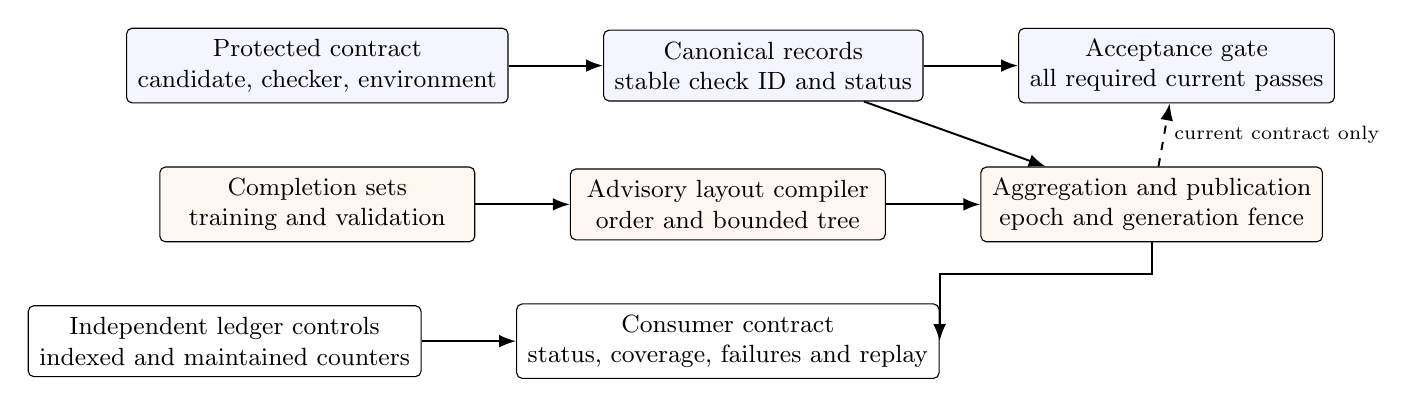
\begin{tikzpicture}[
 >=Latex,box/.style={draw,rounded corners=2pt,align=center,minimum height=9mm,minimum width=40mm,inner sep=4pt,font=\small},
 sem/.style={box,fill=blue!4},lay/.style={box,fill=orange!6},
 arr/.style={->,line width=.7pt},node distance=8mm and 12mm]
 \node[sem] (contract) {Protected contract\\candidate, checker, environment};
 \node[sem,right=of contract] (records) {Canonical records\\stable check ID and status};
 \node[sem,right=of records] (gate) {Acceptance gate\\all required current passes};
 \draw[arr] (contract)--(records);\draw[arr] (records)--(gate);
 \node[lay,below=of contract] (waves) {Completion sets\\training and validation};
 \node[lay,right=of waves] (layout) {Advisory layout compiler\\order and bounded tree};
 \node[lay,right=of layout] (kernel) {Aggregation and publication\\epoch and generation fence};
 \draw[arr] (waves)--(layout);\draw[arr] (layout)--(kernel);
 \draw[arr] (records)--(kernel);
 \draw[arr,dashed] (kernel)--node[right,font=\scriptsize]{current contract only}(gate);
 \node[box,below=of layout] (service) {Consumer contract\\status, coverage, failures and replay};
 \draw[arr] (kernel.south)--++(0,-4mm)-|(service.east);
 \node[box,left=of service] (ledger) {Independent ledger controls\\indexed and maintained counters};
 \draw[arr] (ledger)--(service);
\end{tikzpicture}
\caption{Semantic authority, adaptive representation and the consumer contract.
The compiler cannot modify the protected contract or canonical outcomes.
Both ledger controls and the tree answer the same diagnostic requests.
The diagram is rendered from the included TikZ source; AI assistance is
disclosed in the acknowledgments.}
\label{fig:journal-architecture}
\end{figure*}

\section{Model and Measurement Contract}\label{sec:jmodel}
Let $\mathcal R=(g_0,\ldots,g_{n-1})$ be a nonempty registry of unique semantic
check IDs. A candidate identity
$e=(\mathrm{epoch},\mathrm{snapshot},\mathrm{checker},\allowbreak
\mathrm{environment},\mathrm{registry})$
binds the source and protected acceptance inputs. The epoch increases even
after a return to identical source bytes. Only a trusted runner can supply
final $\PASS$, $\FAIL$ or $\UNKNOWN$ records. Missing, stale, skipped,
incompatible or timed-out evidence does not count as a pass.

A layout $L=(\pi,T)$ maps leaf positions through an exact permutation $\pi$
of semantic indices. Each internal node's children partition its positional
interval without overlap or omissions. Its semantic coverage is $G_L(v)$.
Check execution order is independent of layout order. The acceptance
predicate is, with $E_e(g_i)$ denoting the current matching trusted status,
\begin{equation}\label{eq:accept}
 A(e)=\prod_{g_i\in\mathcal R}\ind\{E_e(g_i)=\PASS\}.
\end{equation}
An observed failure permits rejection before the remaining checks execute,
but supplies no evidence for the unexecuted remainder.

An internal node with $d$ children emits a packet costing
\begin{equation}\label{eq:packet}
 c(d)=H+Sd,\qquad 2\le d\le
 b=\left\lfloor(C-H)/S\right\rfloor.
\end{equation}
The implementation uses $H=512$, $S=320$, $C=3072$ bytes and $b=8$.
Mandatory fields exceeding their slots are rejected. The cap is per packet;
registry manifests are separate control artifacts whose bytes must be charged.

Let $U_{e,a}$ contain the semantic indices whose final records arrive
between two refreshes. The strict-epoch padded cost is
\begin{equation}\label{eq:jcost}
 \ell_e(L)=W(L)+\sum_a\sum_{v\in\operatorname{int}(T)}
 c(d_v)\ind\{G_L(v)\cap U_{e,a}\ne\varnothing\},
\end{equation}
where $W(L)=\sum_vc(d_v)$ constructs an initially unknown tree.
We call $U_{e,a}$ a completion hyperedge. This model charges the full initial
tree and every touched ancestor, rather than using independent activation
probabilities. Persistent refresh models omit a cold build at each event;
each actual installation is still cold and priced.

A layout switch from $i$ to $j$ additionally costs
$M_{ij}=|\mathrm{manifest}(L_j)|+W(L_j)$ when layouts differ.
This is the evaluated uncompressed installation protocol, not a universal
network cost. A format using compression or deltas defines a different
objective and needs its own measurements. Padded packets, compressed
archives, answer traffic, serialized state, RAM and elapsed time remain
separate units.

\medskip\noindent\textit{When this objective applies.}
Neither acceptance nor the evaluated diagnostic API requires a tree.
For those fixed-group queries, maintained counters are the supported service
choice. Equation~\eqref{eq:jcost} instead prices a consumer contract that
explicitly requests refreshed hierarchical capsules with the stated slots.
A remote incremental auditor subscribing to intermediate subtree counts is
a possible contract, not a measured use case or a reason that a flat ledger
cannot emit the same stream. Flat deltas, batching and compressed codecs
would need equal-service comparisons. HACT's local bindings do not provide
Merkle membership proofs or enclave attestation; cryptographic or distributed
consumers require additional protocol design and evidence.

\section{An Information Limit of Pairwise Summaries}
\begin{proposition}[Pairwise probabilities omit subtree-hit information]\label{prop:pairwise}
On three leaves, let $P$ be uniform on
$\varnothing,\{0,1\},\{0,2\},\{1,2\}$ and $Q$ uniform on
$\{0\},\{1\},\{2\},\{0,1,2\}$. Both have singleton probabilities $1/2$,
pairwise joint probabilities $1/4$ and Jaccard affinities $1/3$, but the
triple is touched with probabilities $3/4$ and $1$.
\end{proposition}
This parity fact alone does not imply different global optima: another tree
might dominate in both worlds. The following theorem rules that out under
the affine packet objective.
% Begin inlined generalized_separation.tex
\begin{theorem}[Pairwise information has a sharp optimization penalty]\label{thm:pairwise-optimum}
Let $b\ge3$ be an integer, $H\ge0$, $S>0$, and $\lambda\ge0$.
For $n=b+1$ labeled leaves and internal arities $2,\ldots,b$, define
\begin{align*}
 J_D(T;\lambda)&=\lambda W(T)\\
 &\quad+\E_{U\sim D}\sum_{v\in\operatorname{int}(T)}c(d_v)
       \ind\{G(v)\cap U\ne\varnothing\}.
\end{align*}
There are distributions $P,Q$ with identical singleton and pairwise
probabilities but disjoint globally optimal tree sets, over every feasible
shape and leaf permutation. With $W_2=2H+S(b+2)$,
\begin{align}
 J_P^*&=(1+\lambda)W_2-(H+3S)/4,\label{eq:general-p}\\
 J_Q^*&=(1+\lambda)W_2-(H+2S)/4.\label{eq:general-q}
\end{align}
Any deterministic selector observing only those exact pairwise summaries has
worst-case regret at least $S/4$. The sharp randomized minimax regret is
\begin{equation}\label{eq:minimax-pairwise}
 \frac{S(H+2S)}{4(H+3S)}.
\end{equation}
Sibling orders are treated as equivalent.
\end{theorem}
\begin{proof}
Append $b-2$ anchor leaves, present in every event, to the two three-leaf
parity laws of Proposition~\ref{prop:pairwise}. Every singleton and pairwise
probability agrees, including anchor/parity pairs. An anchor-containing
node is always touched; a node containing only parity leaves is touched
with probability at least $3/4$.

If $I$ is the number of internal nodes, edge counting gives
$W(T)=I(H+S)+Sb$, and the arity cap implies $I\ge2$.
At most two internal nodes contain only the three parity leaves. If there
are two, both are binary; if there is one, its arity is at most three.
Their total price is at most $2c(2)$. Thus for either law and $I\ge3$,
\[
 J_D(T;\lambda)\ge(1+\lambda)W(T)-c(2)/2.
\]
A tree with two internal nodes and a parity-pair child costs
$(1+\lambda)W_2-c(2)/4$ under either law. Every $I\ge3$ lower bound exceeds
that pair tree by at least
\[
 (1+\lambda)(H+S)-c(2)/4
 = (3H+2S)/4+\lambda(H+S)>0.
\]
Such trees are componentwise dominated. With $I=2$, a child containing an
anchor is also dominated by a parity pair. The remaining choices are a
parity pair or the full parity triple. A pair is missed with probability
$1/4$ under either law. The triple is missed with probability $1/4$ under
$P$ and zero under $Q$. Since $c(3)>c(2)$, $P$ uniquely chooses the triple,
whereas $Q$ chooses any of its three pairs. This proves
Equations~\eqref{eq:general-p}--\eqref{eq:general-q}, including construction.

A pairwise-only rule receives identical inputs in both worlds. All other
tree classes are dominated, so a randomized rule need only choose the triple
with probability $q$ and a pair otherwise. Its two regrets are
\[
 r_P(q)=S(1-q)/4,\qquad r_Q(q)=(H+2S)q/4.
\]
The best deterministic choice is a pair, giving worst-case regret $S/4$.
Equating the two affine regrets gives $q^*=S/(H+3S)$ and
Equation~\eqref{eq:minimax-pairwise}. This mixture attains the lower bound.
\end{proof}

The result covers every affine positive-slot price and every fanout at least
three; it is not specific to the artifact's selected byte constants. It
concerns an interface exposing exact population pairwise summaries.
It does not assert equivalence of finite-sample statistical experiments:
joint fluctuations of empirical summary vectors can retain higher-order
information. It neither bounds a method
that retains full waves nor establishes the prevalence of such laws in
software executions. The events describe persistent refresh; a partial
event is not asserted to be a complete strict verification epoch.

% Begin inlined witness_diagram.tex
\begin{figure}[t]\centering
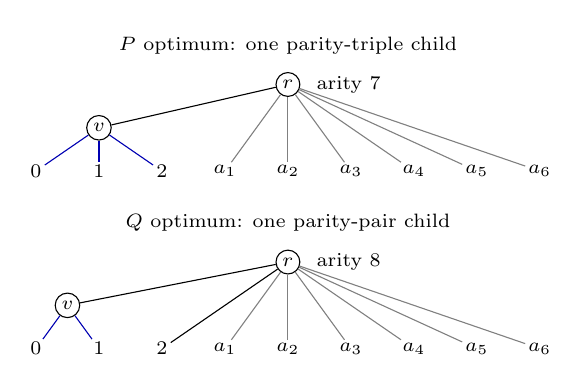
\begin{tikzpicture}[x=.8cm,y=.55cm,every node/.style={font=\scriptsize},
 root/.style={circle,draw,inner sep=1.3pt}, leaf/.style={inner sep=1pt}]
\node at (4,2.9) {$P$ optimum: one parity-triple child};
\node[root] (pr) at (4,2) {$r$};
\node[root] (pt) at (1,1) {$v$};
\node[right] at (4.3,2) {arity 7};
\foreach \x/\lab in {0/0,1/1,2/2,3/a_1,4/a_2,5/a_3,6/a_4,7/a_5,8/a_6}{
 \node[leaf] (p\x) at (\x,0) {$\lab$};}
\draw (pr)--(pt);
\foreach \x in {0,1,2}{\draw[blue!70!black] (pt)--(p\x);}
\foreach \x in {3,...,8}{\draw[gray] (pr)--(p\x);}
\node at (4,-1.2) {$Q$ optimum: one parity-pair child};
\node[root] (qr) at (4,-2.1) {$r$};
\node[root] (qt) at (.5,-3.1) {$v$};
\node[right] at (4.3,-2.1) {arity 8};
\foreach \x/\lab in {0/0,1/1,2/2,3/a_1,4/a_2,5/a_3,6/a_4,7/a_5,8/a_6}{
 \node[leaf] (q\x) at (\x,-4.1) {$\lab$};}
\draw (qr)--(qt);
\foreach \x in {0,1}{\draw[blue!70!black] (qt)--(q\x);}
\draw (qr)--(q2);
\foreach \x in {3,...,8}{\draw[gray] (qr)--(q\x);}
\end{tikzpicture}
\caption{Nine-leaf witness for Theorem~\ref{thm:pairwise-optimum}, with
$H=512,S=320,b=8$. The six anchors $a_i$ are distinct always-present
leaves, each a separate root child. Grouping the parity triple costs
3,856/4,224 refresh bytes under $P/Q$; grouping a pair costs 3,936
under either law. Construction adds 4,224 bytes to both trees.}
\label{fig:pairwise-witness}
\end{figure}
% End inlined witness_diagram.tex

At these prices the deterministic penalty is 80 bytes; randomized minimax
regret is $1440/23\simeq62.609$ bytes, attained by choosing the triple with
probability $5/23$. Integer byte counts are the implementation case; the
theorem also allows real prices. Its zero-header boundary does not change
the serializer's stricter positive-header validation.

An independently implemented exact rational reference checks 39 parameter
cases, including zero headers, fractional construction and header-dominated
prices. It imports no HACT objective or optimizer. The nine-leaf case visits
511 nonempty subset subproblems and 115,462 candidate partitions \emph{across
those subproblems}; it finds one $P$ optimum and three $Q$ optima. Twenty-three
tests include independently listed four-leaf trees and deliberate formula
corruption. These are analytical checks, not additional software workloads.
% End inlined generalized_separation.tex
% Begin inlined strict_separation_summary.tex
\subsection{The separation also occurs in complete epochs}
Persistent refresh is not the only affected regime. Complete epochs
partition all obligations into disjoint nonempty waves.
\begin{theorem}[Complete-epoch information separation]\label{thm:strict-pairwise}
For any fanout $b\ge6$, $S>0$ and $16/11<H/S<28/17$, two laws on six
checks partitioned into three nonempty waves have identical population
singleton and pairwise completion statistics but disjoint unique global
tree optima. Define
\[
 \Delta_P=(28S-17H)/8,\qquad \Delta_Q=(11H-16S)/5.
\]
The sharp deterministic pairwise-only regret is
$\min(\Delta_P,\Delta_Q)$; the sharp randomized minimax regret is
$\Delta_P\Delta_Q/(\Delta_P+\Delta_Q)$.
\end{theorem}
\begin{proof}[Proof sketch; full orbit certificate in the companion analysis]
Let $G=\{0,1,2,3\}$, $O=\{4,5\}$. A block's type $(g,o)$ counts its
members from $G,O$. Let $A=(G,\{4\},\{5\})$, and let $B,C,D$ be uniform
over partitions with block-type multisets respectively
\begin{align*}
 B&:\{(2,1),(2,0),(0,1)\},\\
 C&:\{(2,1),(1,1),(1,0)\},\\
 D&:\{(2,0),(1,1),(1,1)\}.
\end{align*}
Take $P=7A/8+B/8$, $Q=9A/10+C/20+D/20$.
Within-$G$ same-wave probabilities are $11/12$, cross probabilities
$1/32$, and the $O$ pair probability zero in both laws. Uniformly
permuting wave order aligns every window-specific first/second moment.

Contraction strictly improves every nonroot binary or ternary internal
node throughout the stated price interval. With only six leaves, this
reduces all potentially optimal shapes to a flat root or one internal
child. Exact counting over the remaining coverage orbits leaves only
flat and the tree grouping $G$ nondominated. Their cost differences are
$\Delta_P$ and $-\Delta_Q$. Mixing these two actions and equating their
regrets gives the stated minimax result. The companion analysis supplies
the contraction inequalities and all orbit coefficients; an independent
exact reference checks all 2,752 labeled unordered trees.
\end{proof}
At the implemented prices the two wrong-choice penalties are 32 and
102.4 bytes; randomized minimax regret is $512/21$ bytes. This constructed
law has variable-width windows. The next result connects it to fixed-eight
batching without claiming a global 24-leaf optimum.
% End inlined strict_separation_summary.tex
% Begin inlined fixed_batch_summary.tex
\subsection{Fixed-width batches retain a local information gap}
Complete-epoch separation also survives the evaluated flush width.
The following claim concerns two fixed layouts, rather than a global
24-check optimum.
\begin{proposition}[Fixed-eight candidate-class separation]\label{prop:fixed-eight}
For $b\ge6$ and the price interval of Theorem~\ref{thm:strict-pairwise},
two laws on complete 24-check execution sequences have identical population
bivariate completion-rank distributions but opposite preferred choices
in a two-layout class under consecutive batches of eight. Their wrong-choice
penalties remain $\Delta_P,\Delta_Q$, and their class-relative sharp
randomized minimax regret is $\Delta_P\Delta_Q/(\Delta_P+\Delta_Q)$.
\end{proposition}
\begin{proof}[Proof sketch; padding identities in the supplement]
Add 18 distinct fillers to the three-window six-check construction,
uniformly filling each window to eight checks. The probability that an
original check shares a window with a named filler, and that two fillers
share a window, depends only on the original pairwise same-window
probabilities. Thus these probabilities agree under both laws.
Randomly permute the three windows and independently shuffle their members.
For two distinct checks with same-window probability $p$, any specified
pair of distinct ranks has mass $p/(3\cdot8\cdot7)$ within a batch and
$(1-p)/(3\cdot2\cdot8^2)$ between batches. All bivariate rank laws agree.

Place the original six-check subtree and an identical filler-only subtree
under a common root. Compare a flat original subtree with the subtree
grouping $G$. Root and filler costs cancel within each law, preserving
both penalties and the two-action minimax calculation. The supplement
gives the full padding lemma, counting argument and exact conformance
checks.
\end{proof}
At the implemented prices the penalties are 32 and 102.4 bytes, with
randomized regret $512/21$ bytes. The retained reference checks 600
complete 24-check sequences. Neither the rank equivalence nor these finite
checks establish global 24-leaf optimality or equality of joint laws of
empirical pairwise-summary vectors.
% End inlined fixed_batch_summary.tex

\section{Semantics Through Adaptation}\label{sec:jsafety}
A result token carries the candidate epoch, stable ID $g_i$ and a binding
to the identified registry, source, checker and environment. It does not use
a display position as identity. A layout-specific kernel maps each stable
ID to its current position. Migration revokes publication tickets,
increments a monotone generation and reconstructs from canonical records.
Reusing an ordinal cache entry under another permutation is disallowed.

Identical duplicate evidence is idempotent. Conflicting final records in an
epoch revoke authorization: a recorded failure remains a failure, and other
conflicts become unknown. A new epoch is required to resolve them.
Publication tickets additionally bind the layout hash and generation.
Returning to an earlier tree therefore cannot revive its earlier ticket.

\begin{theorem}[Layout-independent local publication]\label{thm:jsafety}
Assume a complete approved registry and dependency identities, a trusted
checker executing immutable identified inputs, collision-resistant bindings
and atomic local epoch/generation checks. For any valid sequence of layouts,
advisory learning outputs and delivered evidence order, authorization implies
$A(e)=1$. Two valid layouts reconstructed from the same canonical record set
have identical root pass/fail/unknown counts.
\end{theorem}
\begin{proof}
A canonical pass requires a current token bound to the same semantic ID and
immutable identities. A permutation is a bijection, so reconstruction moves
each record exactly once without changing its status. Exact child partitions
preserve coverage and counts by induction from leaves to root. Authorization
requires root counts $(n,0,0)$ together with matching current registry, epoch,
layout and generation. Old tickets fail those checks; conflicts prevent a
pass. Advisory layout selection cannot change any canonical outcome or
approved obligation.
\end{proof}

The guard implements conflict persistence and tickets; the claim is local
and conditional. A compromised checker, incomplete suite or omitted
dependency invalidates broader claims. There is no attestation or OS sandbox;
an external merge service must atomically bind the verified candidate to its
integration head.

The implementation hashes protected input \emph{sets} to detect additions,
changes and deletions, and checks source manifests around snapshotting and
verification. Snapshots and detailed evidence lie outside the candidate's
write scope; the worker receives a bounded result card. The artifact tests
stale tokens, conflicts, migration, coverage and source mutation. Passing
tests do not establish that predicates cover all program behavior.

\section{Bounded Full-Wave Compilation}\label{sec:jcompiler}
\subsection{Exact fitting at a fixed order}
For a fixed order $\pi$, training epochs define interval weights
\begin{equation}\label{eq:jweights}
 r_\pi(i,j)=1+\frac1m\sum_{e=1}^m\sum_a
 \ind\{U_{e,a}\cap G_L(i,j)\ne\varnothing\}.
\end{equation}
The one charges construction per strict epoch. In a persistent refresh study
that term is omitted explicitly.
Let $D(i,j)$ be the best subtree cost and $F_k(i,j)$ the best ordered
$k$-component forest. Infeasible states are infinite:
\begin{align}
 D(i,i)&=0,\qquad F_1(i,j)=D(i,j),\nonumber\\
 F_k(i,j)&=\min_{i+k-2\le u<j}
       \{F_{k-1}(i,u)+D(u+1,j)\},\nonumber\\
 D(i,j)&=\min_{2\le k\le\min(b,j-i+1)}
       \{r_\pi(i,j)c(k)+F_k(i,j)\}.\label{eq:dp}
\end{align}
The recurrence enumerates every root arity and contiguous partition.
Induction on interval length proves exactness for the supplied nonnegative
weights, conditional on order. It uses $O(bn^3)$ time and $O(bn^2)$ space.
This specializes classical alphabetic-tree optimization~\cite{alphabetic};
it is not a global permutation optimizer or an optimum for compressed logs.

% Begin inlined bounded_refinement.tex
\subsection{A bounded restricted optimizer}
The historical practical method fits Jaccard affinities, obtains an
average-linkage order and groups consecutive leaves into compact blocks of
at most eight. Full-wave validation retains either the incumbent or the
learned compact layout. The new optional method refines \emph{maximal existing
subtrees} containing at most $s$ leaves. Each selected subtree is disjoint
from the others. It keeps the order and that subtree's leaf interval, solves
Equation~\eqref{eq:dp} on projected training waves, and accepts a replacement
only if the complete integer training objective strictly decreases.
All larger ancestors remain unchanged; ties retain the incumbent subtree.

\begin{proposition}[Restricted exactness and bounded refinement]\label{prop:jrefine}
For a fixed order and fixed disjoint refinement intervals, independent exact
fitting minimizes training cost over trees obtained by replacing only those
subtrees. Retaining the incumbent on ties gives nonincreasing integer
training cost. For intervals of sizes $m_i\le s$, the DP work is at most
$O(bns^2)$ with $O(bs^2)$ peak DP storage, apart from input projection,
cost computation and ordering.
\end{proposition}
\begin{proof}
All ancestor contributions depend only on the unchanged coverage and arity.
The mutable objective is the sum of independent interval objectives, so
minimizing each minimizes the restricted sum. The incumbent is feasible in
every subproblem. Since $\sum_im_i\le n$,
$\sum_im_i^3\le s^2\sum_im_i\le ns^2$. Sequential solution gives the stated
storage bound. Integer rescoring rejects a numerically nonimproving DP
replacement.
\end{proof}

The implementation uses float64 inside the existing recurrence; exactness
is to numerical precision. Independent integer rescoring establishes
monotonicity, not exact rational optimality for every large instance.
Independent literal-tree enumeration checks tiny cases. Every leaf remains
present exactly once and all packet arities remain feasible.

The primary frozen cap is $s=32$; $64$ is a secondary sensitivity.
A full compact8 ancestor above eight eight-leaf blocks covers $8^2=64$
leaves. With $s=32$, its blocks are solved separately: no replacement can
cross a block boundary, merge adjacent blocks or change that ancestor.
Cap64 opens this first cross-block topology decision. Ragged boundary
subtrees can have other sizes; the actual largest solved interval is reported.
This interaction explains why cap32 often ties while the prespecified cap64
sensitivity improves. It does not change the frozen primary endpoint or
isolate a higher-order causal effect.
Dense pairwise ordering still has quadratic storage and approximately
$O(n^2\log n)$ heap work. It can dominate bounded refinement and is admitted
separately under the resource budget.
% End inlined bounded_refinement.tex
\subsection{A bounded sparse ordering proposal}\label{sec:sparse}
The post-review prototype stores positive Jaccard pair counts from training
waves and proposes a compact order by a deterministic maximum-spanning
forest~\cite{kruskal} and depth-first traversal. For $W$ waves of width at most $w$, it
uses $O(n+E)$ ordering storage, where $E\le W\binom w2$ is the number of
distinct positive pairs; sorting costs $O(E\log E)$ arithmetic operations.
An explicit edge budget rejects oversized inputs. This replaces the dense
ordering heuristic, not the full-wave objective or the verifier. Validation
chooses between original and sparse compact layouts using exact touched-node
costs; the separate ancestor-scoring index takes $O(n\,\mathrm{height})$
references. No cap64 fit is included in the large-registry follow-up.
% Begin inlined exchangeable_optimum.tex
\subsection{An exact global baseline under completion symmetry}\label{sec:symmetry}
The information lower bound is a worst-case statement. A structured null
regime admits a global optimum without learning co-activity. Fix nonempty
batch sizes $w_1,\ldots,w_q$ summing to $n$. Complete a uniformly random
permutation of the registry and partition it into those consecutive batches.
For any semantic coverage $G$ of size $s$, the expected number of touched
waves is
\begin{equation}\label{eq:symmetry-weight}
 r_n(s)-1=\sum_{a=1}^q\left(1-
       \frac{\binom{n-s}{w_a}}{\binom n{w_a}}\right),
\end{equation}
where a binomial coefficient with upper argument smaller than its lower
argument is zero. The one in $r_n(s)$ charges the cold build.
No independence among checks or waves is assumed. The formula also follows
from exchangeability conditional on the declared ordered batch sizes.

Let $D(s)$ minimize expected subtree cost for $s$ leaves, using the
\emph{full-registry} weights $r_n(s)$. Let $F_d(s)$ minimize the sum of
$d$ nonempty child-subtree costs, with infeasible states infinite:
\begin{align}
 D(1)&=0,\qquad F_1(s)=D(s),\nonumber\\
 F_d(s)&=\min_{1\le t\le s-d+1}\{D(t)+F_{d-1}(s-t)\},\nonumber\\
 D(s)&=\min_{2\le d\le\min(b,s)}
        \{r_n(s)c(d)+F_d(s)\}.\label{eq:symmetry-dp}
\end{align}

\begin{theorem}[Global optimality under exchangeability]\label{thm:symmetry}
For the declared exchangeable completion law, Equation~\eqref{eq:symmetry-dp}
minimizes the expected strict-epoch padded cost over every feasible tree
shape and leaf permutation. After computing the weights, it uses
$O(bn^2)$ arithmetic operations and $O(bn)$ states. With integer packet
prices it can be evaluated exactly using a common denominator and integer
numerators; arithmetic bit complexity is additional.
\end{theorem}
\begin{proof}
Any batch is a uniform $w_a$-subset of the full registry. Its probability
of missing $G$ is the binomial ratio in~\eqref{eq:symmetry-weight}.
Linearity of expectation gives each internal node the contribution
$r_n(s)c(d)$, depending only on its coverage size and arity. Conditioning
on a root's arity and nonempty child sizes leaves the sum of independent
optimization subproblems; probabilistic independence is unnecessary.
Induction on $s$ proves the forest and tree recurrences enumerate all
possible shapes. Relabeling leaves changes no expected contribution, so
canonical depth-first labels attain the unrestricted permutation optimum.
Every forest transition scans at most $s$ splits for each $(d,s)$,
giving $O(bn^2)$ work and $O(bn)$ stored costs/splits. Multiplying all rational
weights by their common denominator preserves every comparison and tie.
\end{proof}

Consequently, if a future epoch retains this exchangeable law conditional
on the training data and selected layout, no training-dependent selection
improves its expected padded cost below $D(n)$. Condition on that selection:
each fixed tree costs at least $D(n)$, then average over training. Independent
training and future epochs suffice; unconditional symmetry alone does not
exclude training information that predicts the future completion pattern.
This gives a concrete null baseline against which to test learning.
Graham, Li and Yao already optimize batch-update key trees using cardinality
states under independent Bernoulli replacements~\cite{graham2007}.
Our fixed-size, without-replacement law, affine capped packet prices and
per-epoch cold charge specify a different instance; the size-state principle
is established. Neither a shuffled dispatch queue nor a good
fit to one trace establishes exchangeable completion times. Violating the
model removes the global-optimality guarantee, so we also score this baseline
on the frozen structured traces and retain its losses. The objective excludes
query service, compilation seconds and installation manifests; those remain
separate lifecycle ledgers. The model-derived layout is an optional advisory
candidate and does not change the acceptance registry or runtime policy.
% End inlined exchangeable_optimum.tex
\subsection{Validation and adoption}
Training fixes a finite catalogue containing the incumbent first.
Validation observes complete waves and selects the minimum padded cost,
retaining the incumbent on ties. The historical method remains unchanged;
the refined catalogue is optional.

Empirical validation alone gives no deployment guarantee. The following
rule uses independent calibration and an explicit shift allowance.
Repeated suite runs do not establish those sampling assumptions.

% Begin inlined adoption_summary.tex
\subsection{Conditional adoption with lifecycle costs}\label{sec:adoption}
A training-fitted catalogue is frozen before independent calibration.
All layouts share the registry and packet contract. Relative to incumbent
$L_0$, aggregate packet-price differences by semantic coverage:
\[
a_{jG}=\sum_{v:G_{L_0}(v)=G}c(d_v)
       -\sum_{v:G_{L_j}(v)=G}c(d_v).
\]
Shared packets cancel. If $h_e(G)$ counts intersecting waves, the
strict-epoch saving $d_j(e)=\ell_e(L_0)-\ell_e(L_j)$ is
\begin{equation}\label{eq:paired-saving}
d_j(e)=a_{j0}+\sum_Ga_{jG}h_e(G),\quad a_{j0}=\sum_Ga_{jG}.
\end{equation}
For an epoch partitioning $n$ checks into exactly $q$ nonempty waves
of size at most $w$, with $q\le n\le qw$, a coverage of size $s$ satisfies
\begin{equation}\label{eq:hit-envelope}
l_G=\max\{\lceil s/w\rceil,q-(n-s)\}
 \le h_e(G)\le u_G=\min(s,q).
\end{equation}
Every untouched wave needs a distinct check outside $G$; in particular
$h_e(\mathcal R)=q$. Conservative bounds on the entire declared support are
\begin{align*}
A_j&=a_{j0}+\sum_G\min\{a_{jG}l_G,a_{jG}u_G\},\\
B_j&=a_{j0}+\sum_G\max\{a_{jG}l_G,a_{jG}u_G\}.
\end{align*}
Thus $d_j(e)\in[A_j,B_j]$ and $R_j=B_j-A_j$.
Different coverages' extrema need not be jointly attainable.

\begin{proposition}[Exact population score identification]\label{prop:summary-span}
On finite epoch support $\Omega$, an interface exposing only
$\E_P\phi_1,\ldots,\E_P\phi_p$ determines $\E_Pd_j$ for every law $P$
if and only if $d_j\in\operatorname{span}\{1,\phi_1,\ldots,\phi_p\}$
on $\Omega$.
\end{proposition}
\begin{proof}[Proof sketch; full identification argument in the supplement]
Span membership gives affine recovery. Otherwise a signed vector
orthogonal to $1,\phi_1,\ldots,\phi_p$, but not $d_j$, gives two
normalized nonnegative laws with identical exposed moments and different
expected scores.
\end{proof}
For a frozen catalogue, exact paired scoring needs only each accumulated
integer score and an epoch count: $O(K)$ counters besides coefficients
and one epoch's masks. Acceptance records and required raw provenance
remain separate. Exact score recovery alone does not imply argmin recovery.

\begin{theorem}[Conditional expected lifecycle benefit]\label{thm:adoption}
Condition on training and the frozen catalogue of $K\ge1$ candidates,
support, $0<\delta<1$, TV radius $0\le\rho\le1$, horizon $h\ge1$ and
nonnegative installation costs $I_j$, all specified before calibration.
Suppose the $m\ge1$ calibration epochs are IID from $P$ and independent
of fitting. With paired mean $\bar d_j$, define
\begin{align}
t_j&=R_j\sqrt{\frac{\log(K/\delta)}{2m}},\nonumber\\
g_j&=\max\{A_j,\bar d_j-t_j-\rho R_j\}-I_j/h.
\label{eq:adoption-lower}
\end{align}
With probability at least $1-\delta$ over calibration, simultaneously
for all candidates and every future law $Q$ on the same support with
$\operatorname{TV}(P,Q)\le\rho$, $h\,\E_Qd_j-I_j\ge h g_j$.
Adopting only a candidate with $g_j>0$, otherwise retaining $L_0$,
certifies a conditional positive expected padded-byte benefit.
\end{theorem}
\begin{proof}
One-sided Hoeffding bounds and a union bound give
$\E_Pd_j\ge\bar d_j-t_j$ simultaneously~\cite{hoeffding,learntest}.
For $\operatorname{TV}(P,Q)=\sup_E|P(E)-Q(E)|$,
a function of range width $R_j$ changes expectation by at most
$\rho R_j$. Also $\E_Qd_j\ge A_j$ on the same support.
Subtract installation and multiply by $h$. Zero-width scores are
constant, so the conclusion also holds when $R_j=0$.
The supplement gives the full argument and implementation contract.
\end{proof}
This certifies neither realized savings, elapsed time nor acceptance.
The sampling design and radius require external justification. Deployment
outside the support, refitting on calibration, or repeatedly changing
catalogues needs new accounting. The implementation binds the plan to a
digest and requires sampling/freeze provenance; missing evidence returns
$\UNKNOWN$. Installation is charged once; compilation and consumer
utility remain separate admission tests.
% End inlined adoption_summary.tex

\begin{table}[t]\centering\footnotesize
\caption{Established ingredients and the contribution claimed here.}
\label{tab:novelty}
\begin{tabularx}{\columnwidth}{@{}p{.31\columnwidth}X@{}}\toprule
Established ingredient & Claim under the HACT contract\\\midrule
Alphabetic and batch-update tree DP & Exact fixed-order reference and global size-state optimum under declared exchangeability; both specialize established DP principles.\\
Pairwise clustering and hypergraphs & Explicit indistinguishable laws with disjoint global optima and sharp regret; fixed-batch local extension.\\
Epochs, identities and fencing & Conditional composition preserving the approved all-check acceptance predicate during representation migration.\\
Subtree optimization and validation & Bounded full-wave refinement; conditional paired-cost adoption under externally justified sampling and shift assumptions.\\
Ledgers, counters and common codecs & Controlled comparison separating representation gains from service costs, including losses.\\\bottomrule
\end{tabularx}
\end{table}

Compilation, selection and installation are separately charged. A saving
of $g$ bytes per epoch repays installation $I$ only when $h g>I$; including
compilation seconds requires a measured unit conversion. Padded bytes imply
no token or agent speedup. The supplement's empirical-Bernstein alternative
has a finite-range term exceeding the constructed mean saving at $m=50$;
variance sensitivity is not an established remedy in this example.

\section{Evaluation Protocol}\label{sec:jevaluation}
The evaluation asks four questions:
\begin{enumerate}
\item Can the information limit and semantic invariant be checked independently?
\item Does bounded full-wave refinement improve over compact baselines?
\item Does a tree repay its full service costs against strong ledgers?
\item Which observed workload and resource boundaries limit adoption?
\end{enumerate}

\subsection{Evidence cohorts and frozen decisions}
Freezes are internal source/input records, not external preregistration;
cohorts and endpoint roles remain fixed. The compiler study reuses 27 frozen
synthetic train/validation/held-out cells and twelve archived candidate traces
from three projects, preserving their provenance.

The public cohort is a declared convenience sample: Click 8.2.1,
Jinja 3.1.6, Packaging 25.0, Pluggy 1.6.0, attrs 25.3.0 and
ExceptionGroup 1.3.0. Tags resolve to commits, tracked files are hash-bound,
and imported modules are checked against clean checkouts. Five fresh runs of
each unchanged upstream suite are assigned in advance: runs 0--1 training,
2 validation and 3--4 held out. Final phases and arrival order are recorded;
at most eight successive completions form a wave, as in the historical protocol.
These test executions are not independent source changes, natural-bug repairs
or agent episodes.

The registry is a sorted ID set; collection, scheduling and completion orders
are retained separately. A collection-order instrumentation correction is
recorded before cost analysis, with raw inputs preserved. Skips, xfails and
xpasses remain $\UNKNOWN$; ordinary failures are retained, environmental
failures disclosed, and exclusions and resource admission explicit.

Methods and receipts are frozen before held-out costs are opened. The six
requested projects, five admitted to optimization, are case-level units;
checks, cached requests, repeats and replays do not enlarge the sample.
We report per-project measurements without population-level superiority tests.

\subsection{Controls, estimands and uncertainty}
The primary compiler endpoint compares refined and historical compact
selection on strict-epoch padded bytes, including construction. Original
and pairwise orders are compared before and after refinement at the
\emph{same order}, separating topology from ordering without identifying
higher-order information as the cause of a gain. The exact parity case checks
use of full waves when pairwise affinities agree; it is analytical conformance.

The service endpoint sums local operations over a retained trajectory:
construction, eight-completion ingests, query aggregation, encoding and
decoding. Input snapshot preparation and the independent oracle are outside
both timers; checker execution is separate. Initial, intermediate and final
snapshots receive status, failure, unfinished, coverage and replay queries,
each cold and repeated warm. This layout-independent sequence is a controlled
integration workload, not observed production demand.

Controls are the original indexed ledger and a stronger ledger maintaining
fixed-group status counters. Tree and ledger query maintained state; a third
computation answers from raw records. Answers, missing-obligation sets and
epochs must match or performance promotion halts. Identical bounded pages
and deterministic DEFLATE imply equal answer bytes. Serialized state and
logical update bytes remain separate from wire traffic and resident memory.

Three whole-trajectory executions use seeded randomized arm order. Timings
describe this host and workload, not additional projects. Paired per-case
summaries retain unfavorable cases without significance claims from correlated
queries. Per-arm timeouts remain $\mathrm{UNKNOWN}$, not zero-cost successes.

% Begin inlined v12_followup_protocol.tex
\subsection{Review-motivated follow-up protocols}
Two separately frozen follow-ups address weaknesses found in the original
study. Both retain the original layouts and all unfavorable observations.
First, each of the five admitted release suites executes under three fixed
seeds crossed with two dispatch policies: shuffling test-file groups while
preserving within-file order (primary), and shuffling individual items
(secondary). These are actual complete pytest processes, not permutations
of recorded outcomes. Registry equality, scheduled versus actual completion
order, imported source origins and pre/post source hashes are checked.
Fixed-eight waves from each completed execution are priced by an independent
literal-tree evaluator. No layout is refitted, and a registry, timeout or
provenance failure makes a case VOID or UNKNOWN. The method retains both
the original compact and historical selected comparators.

Second, byte-count instrumentation in the original service serializes
maintained state and records inside the timers. A new eight-arm campaign
crosses all four services with original and observer-disabled implementations
on the same ten admitted trajectories, with three seeded randomized-order
repeats. Observer-disabled subclasses remove serialization used solely to
measure byte counters; functional record copies, validation, evidence digests,
kernel refresh and packet serialization, caches and answer-codec work remain.
The old observations are not retroactively corrected. New semantic/wire
oracle checks precede interpretation of timings. Full duplicate-aware
package inventories and source/input hashes are frozen for both follow-ups.

OpenAI Codex supported implementation, proof checking, experiment orchestration
and analysis; checks by separate AI agents are automated checks, not human
peer review. Numerical tables and plots derive from retained JSON observations
through the supplied Python scripts. The v11 figure code was assisted by
Codex; the v12 analysis and revision also used Codex. Exact model-version
identifiers were not captured in the experiment manifests.
The raw observations, code and protocols permit verification without an AI
service. No language model participates in the measured service operations.
% End inlined v12_followup_protocol.tex

\section{Results and Applicability}\label{sec:jresults}
\subsection{Theory and semantic conformance}
The independent rational reference verifies 39 parameter cases for
Theorem~\ref{thm:pairwise-optimum}. Independently listed literal trees,
partition-count checks and formula-tampering tests reduce shared-code risk.
The mathematical proof covers arbitrary admissible fanout and prices;
finite enumeration checks its implementation and boundary examples, rather
than substituting for the proof. Semantic regression tests cover stale
tickets, conflicts, permutations and epoch/generation transitions.

\subsection{Historical representation results and new ablation}
Frozen clustered synthetic workloads yield held-out padded-byte savings of
23.43\%, 10.75\% and 5.56\% at 128, 512 and 1,024 checks relative to the
original balanced baseline. Independent/global controls show essentially
no systematic benefit. Re-encoding the twelve archived candidates changes
compressed hierarchical streams by 4.36--41.84\%; these are within-format
results and do not establish service superiority.

The new bounded-refinement experiment is more restrictive than a global
optimizer. At cap 32, all 27 historical cells tie the validation-selected
compact catalogue. At cap 64, 26 tie and one saves 0.00762\% on held-out
padded bytes. The isolated sensitivity gain is not a practical breakthrough
or a confirmatory higher-order effect. Independent dictionary-tree
reconstruction verifies the reported objectives without calling the
producer's cost helper. The archived direct-wave heuristic also showed
no gain. These results favor retaining a compact incumbent unless
independent evidence pays for a more expensive compiler.

% Begin inlined v12_journal_results.tex
% V12 projection; v11 source observations and generated table remain immutable.
\subsection{New public-software executions}
Thirty fresh process runs on six upstream projects record 151,380 check
executions. Table~\ref{tab:v11-cohort} reports one held-out run per project;
the second has the same counts. These counts are execution observations,
not independent projects. Only five projects (25 runs, 16,640 check
executions) are admitted to the compiler comparison. All five have identical
completion orders and ordered wave partitions across runs 0--4. Thus the
held-out costs measure repetition of observed completion patterns, not
prediction of new patterns. attrs' 33 failures concern this environment
(including mypy compatibility) and are retained without calling them
upstream bugs. Skips, xfails and xpasses remain unknown.

\begin{table}[t]\centering\footnotesize
\caption{New complete suites. Counts per held-out run; five runs per project.
P/F/U are PASS/FAIL/UNKNOWN.}\label{tab:v11-cohort}
\begin{tabular}{@{}lrrrr@{}}\toprule
Project & Checks & P & F & U\\\midrule
Click & 761 & 739 & 0 & 22 \\
Jinja & 909 & 909 & 0 & 0 \\
Packaging & 26,948 & 26,948 & 0 & 0 \\
Pluggy & 124 & 124 & 0 & 0 \\
attrs & 1,432 & 1,391 & 33 & 8 \\
ExceptionGroup & 102 & 91 & 0 & 11 \\
\bottomrule\end{tabular}
\end{table}

Raw collection order varied in Packaging. Before any layout-cost analysis,
a dated correction created separate canonical-registry copies, retaining
the raw records and every scheduled/completed ID unchanged. Jinja's missing
Trio test dependency was repaired before its five retained runs; the original
failed attempt is preserved. Source files remain hash-verified. The original
environment identifier binds Python/platform, not all dependencies.
A post-hoc inventory records the repair and duplicate package metadata;
it cannot retroactively establish a complete contemporaneous environment
identity. Each representation comparison still uses the same persisted
input trace.

\subsection{Held-out topology costs}
Table~\ref{tab:v11-gains} compares frozen refined selections to historical
compact selection. The primary cap32 method improves two of five admitted
project cases and ties three. The cap64 results were designated secondary
before collection; they do not replace the primary endpoint. Both methods
are fitted on runs 0--1, selected on run 2 and scored on runs 3--4.
All selected layouts were hash-frozen before those held-out costs were opened.
\begin{table}[t]\centering\footnotesize
\caption{Held-out padded-byte reduction (\%) relative to the historical
compact catalogue. Construction is included. UNKNOWN is not a tie.}
\label{tab:v11-gains}
\begin{tabular}{@{}lrr@{}}\toprule
Project & Cap32 primary & Cap64 secondary\\\midrule
Click & 1.493 & 17.219 \\
Jinja & 0.177 & 15.996 \\
Packaging & \multicolumn{2}{c}{UNKNOWN} \\
Pluggy & 0.000 & 18.695 \\
attrs & 0.000 & 0.000 \\
ExceptionGroup & 0.000 & 18.690 \\
\bottomrule\end{tabular}
\end{table}

The positive secondary reductions range from 16.00\% to 18.69\%; attrs
retains its incumbent. The gain is a measured topology-refinement effect
at the stated order, not a causal demonstration that higher-order information
alone explains it. Figure~\ref{fig:v11-boundaries} separates this representation
endpoint from service time.

Packaging has 26,948 declared checks. One dense float64 affinity matrix
alone would require about 5.81\,GB (5.41\,GiB); dictionary/heap clustering
needs more. The compiler therefore records optimization UNKNOWN under its
2\,GiB campaign budget, retains every ID and supplies an explicitly labeled
compact fallback only for conformance/scaling records. It is excluded from
the five-project compiler comparison rather than being counted as a tie.

\subsection{Transfer to historical-source regressions}
An additional frozen plan selects eleven real upstream fix commits by
syntax and history, transplants their parent production modules into
isolated release snapshots, and runs unchanged release tests with
stop-on-first-failure. Nine cases execute; eight preserve the release
registry. Two startup incompatibilities and one changed semantic ID set
are VOID for paired analysis. One matching Packaging case remains UNKNOWN
because fitting was not admitted. The seven measured transfers yield
two primary wins, three ties and two losses. In particular, Click's
primary layout costs 2.09\% and 2.58\% more than the historical compact layout
on its two partial trajectories. The retained all-pass Jinja case is
unrevealing, rather than excluded.

These are exploratory source transplants under a newer fixed test contract,
not executions of each native historical parent suite or a certified
natural-bug benchmark. They share project tests and supply no extra
independent project replication. No source-transfer outcome changes the
frozen layout. The losses demonstrate that training monotonicity and a
successful repeated-snapshot holdout do not ensure benefit after a source
or stopping-pattern change.

\subsection{Whole-trajectory service accounting}
The original comparison admits ten traces from five projects at the fixed 2,048-check
service budget; both complete Packaging inputs remain UNKNOWN without
subsampling. It executes four arms, three randomized-order repeats and
cold/warm queries at initial, intermediate and final snapshots.
All 5,040 service/oracle answer checks agree,
including exact epoch and missing-check disclosure. Each arm delivers the
same complete answer bytes under the common deterministic codec.

\begin{table}[t]\centering\footnotesize
\caption{Local service operation time (ms), mean of two per-case medians over
three whole-trajectory timing repeats. Builds, all ingests, queries and
codec work are included. Layout fitting is reported separately.
No network or agent inference occurs.}\label{tab:v11-time}
\begin{tabular}{@{}lrrr@{}}\toprule
Project & Indexed & Counters & HACT32\\\midrule
Click & 392.1 & 422.4 & 996.3 \\
Jinja & 555.0 & 527.4 & 1236.8 \\
Pluggy & 38.5 & 37.6 & 56.4 \\
attrs & 1067.1 & 1169.5 & 2833.9 \\
ExceptionGroup & 30.2 & 29.1 & 41.8 \\
\bottomrule\end{tabular}
\end{table}

These original timings include observational serialization for byte
counters, including whole-state serialization at every ingest. They measure
the instrumented prototype rather than isolated functional service costs.
All 30 matched timing-repeat HACT32/counter ratios exceed one
(range 1.216--2.850); repeated timings are descriptive, not independent
project replications. The separately frozen observer ablation below
measures the effect of this instrumentation.

The selected HACT service is slower than the maintained-counter ledger in
every admitted project case. Its ratio of mean case-median operation times
ranges from 1.44 to 2.42 on this host. Additional layout fitting and manifest
admission cannot turn those observed service losses into a positive
end-to-end speedup. The table times precompiled service execution and does
not hide fitting inside common checker time. Compiler receipts retain
separate one-time fit/selection measurements; their concurrent collection
load makes them descriptive rather than controlled speedup estimates.
The outcome supports a maintained ledger as the initial service baseline
for these requests, while preserving the distinct within-format packet
savings above.

\begin{figure*}[t]\centering
\includegraphics[width=.96\textwidth]{hact_inline_figure.pdf}
\caption{Different endpoints lead to different adoption decisions.
Left: primary and prespecified secondary held-out padded-byte savings.
Right: original instrumented precompiled service time of primary HACT divided by the
maintained-counter ledger; values above one are slower. Packaging is
UNKNOWN under resource admission and is not plotted as zero.}
\label{fig:v11-boundaries}
\end{figure*}

% Begin inlined v12_followup_results.tex
\subsection{Controlled dispatch-shift transfer}
The new campaign contains 36 complete suite executions and 20,580 check
executions. Six initial ExceptionGroup runs are VOID for cost analysis:
the profiler observed an ignored build-generated version module absent from
the frozen tracked-source inventory. Their raw records are retained. A
separate child protocol freezes that module before rerunning all six
predeclared schedules, without changing tests, seeds, layouts or endpoints.
The resulting admitted comparison has 30 executions and 19,968 checks over
five projects; it does not silently reclassify the original exclusions.
All admitted runs retain the original registry and status counts, including
attrs' environment-related failures.

\begin{table}[t]\centering\footnotesize
\caption{Primary cap32 padded-byte reduction (\%) under controlled dispatch
shifts relative to historical compact selection. Ranges span the three
fixed seeds; negative values are losses. No refitting.}
\label{tab:v12-shifts}
\begin{tabular}{@{}lrr@{}}\toprule
Project & File groups & Individual items\\\midrule
Click & -4.85 to -3.33 & -9.01 to -8.94 \\
Jinja & 0.15 to 0.17 & -0.12 to -0.07 \\
Pluggy & 0.00 & 0.00 \\
attrs & 0.00 & 0.00 \\
ExceptionGroup & 0.00 & 0.00 \\
\bottomrule\end{tabular}\end{table}

Against the historical selected comparator, file-group shuffling gives
three primary wins, nine ties and three losses; item shuffling gives zero
wins, nine ties and six losses. The comparison unit here is a scheduled
process, not an independent project. The small Jinja file-group gain survives,
whereas Click loses under both shifts. The three ties are projects whose
primary selection did not change. This directly limits the inference from
the repeated-pattern holdout. Every seed, all four frozen layouts, the
original compact comparison and secondary cap64 prices are retained in
the artifact. Neither the intervention nor the analytical witness identifies
natural deployment prevalence or a causal higher-order benefit.

\subsection{Service costs with byte observers disabled}
The separate ablation completes 240 arm executions: ten held-out traces,
three repeats and eight arms. All 10,080 raw-oracle/common-codec answer
checks agree; the two complete Packaging traces remain UNKNOWN under the
unchanged service budget. Table~\ref{tab:v12-observer} compares the same
primary layout to the maintained-counter ledger within each new timing block.

\begin{table}[t]\centering\footnotesize
\caption{Observer ablation. Disabled columns are mean case-median operation
times (ms); ratios compare HACT32 with counters in the same campaign.
Off=byte observers disabled (HACT32 ms / Counter ms at left);
on=original instrumentation in separate paired executions.}
\label{tab:v12-observer}
\begin{tabular}{@{}lrrrr@{}}\toprule
& \multicolumn{2}{c}{Observers off (ms)} & \multicolumn{2}{c}{HACT/counter}\\
Project & Counter & HACT32 & Off & On\\\midrule
Click & 137.9 & 429.2 & 3.11 & 2.16 \\
Jinja & 140.3 & 446.1 & 3.18 & 2.23 \\
Pluggy & 23.0 & 37.1 & 1.61 & 1.45 \\
attrs & 261.3 & 924.9 & 3.54 & 2.64 \\
ExceptionGroup & 20.3 & 39.0 & 1.92 & 1.43 \\
\bottomrule\end{tabular}\end{table}

Removing observational serialization reduces absolute service time but
does not reverse the comparison. Primary HACT is slower than counters
in every paired timing block under both instrumentation states. With
observers disabled, the project ratios of mean case medians range from
1.61 to 3.54; individual paired-block ratios range from
1.135 to 4.630. These are descriptive host-specific
ranges, not confidence intervals. The disabled variant retains functional
packet serialization, evidence digests, record copies, validation, caches
and codec round trips. It is a controlled prototype ablation, not an optimized
production implementation. The negative service result therefore survives
the identified observer-cost confound for this demand.
% End inlined v12_followup_results.tex
% End inlined v12_journal_results.tex
% Begin inlined v13_results.tex
% Generated by experiments_v13.report from audited retained v13 numbers.
\subsection{Exact scoring interfaces and conditional adoption}
Proposition~\ref{prop:summary-span} separates two requirements:
retaining enough information to fit a new layout, and scoring a frozen
catalogue. On all 90 three-block partitions of six checks, an exact
rational calculation gives rank 16 for the constant and fifteen pairwise
same-window features, rising to 17 after appending the grouped-versus-flat
paired score. A single additional score feature suffices for this fixed
comparison. The rank calculation verifies the scoring statement; the
earlier global-optimum theorems supply the stronger optimization obstruction.

The independent literal-tree scorer agrees with the paired implementation
and structural envelope in 247,680 comparisons: all 2,752 labeled unordered
six-leaf trees against flat, across all 90 complete three-window partitions.
The checks include arbitrary display orders; four-leaf regressions also
enumerate every feasible width/window-count combination. These are exact
analytical conformance checks, not new software projects.

For the complete-epoch witness at the implemented prices, the grouped
layout saves an expected 32 bytes under $P$ and loses 102.4 under $Q$.
Its paired support interval is $[-3328,256]$, of width 3,584 bytes;
bounding both whole costs separately gives width 22,784. Their squared
width ratio is approximately 40.41, a bound-dependent sample-complexity
comparison, not measured task acceleration.

We fix the two layouts, $\delta=0.05$, zero shift, a 1,000-epoch horizon
and 3,684 additional pre-horizon installation bytes before a seeded
synthetic calibration study. Twenty seeds per law use nested prefixes of
100,000 draws. Table~\ref{tab:v13-adoption} reports conditional-adoption
counts for Equation~\eqref{eq:adoption-lower}; whole-cost bounds use the
same observed paired means and installation ledger. The direct streaming
API agrees with the intended positive scenario and retains the incumbent
when the declared TV radius rises to 0.01. No population significance or
empirical confidence coverage is inferred from these twenty seeds.

\begin{table}[t]\centering\small
\caption{Synthetic conditional adoption counts. Repeated prefixes are
dependent within seed. Under $Q$, neither bound adopts at any listed size.}
\label{tab:v13-adoption}
\begin{tabular}{@{}rrrr@{}}\toprule
Calibration $m$ & $P$: paired & $P$: whole & $Q$: paired\\\midrule
100 & 0/20 & 0/20 & 0/20\\
1,000 & 0/20 & 0/20 & 0/20\\
10,000 & 1/20 & 0/20 & 0/20\\
100,000 & 20/20 & 0/20 & 0/20\\
\bottomrule\end{tabular}
\end{table}

Even with infinite calibration and no installation charge, a mean saving
of 32 bytes cannot make this lower bound positive for
$\rho\ge32/3584=1/112$. This is the limit of this conservative certificate,
not a sharp minimax drift tolerance or an estimate of software-workload drift.
All five admitted public-project rows remain $\UNKNOWN$: repeated
snapshots and controlled schedule interventions supply neither the required
independent natural calibration nor an externally justified deployment TV
bound. Packaging's resource exclusion is retained separately. This new
analysis neither changes the historical 3/18/9 shift outcomes nor establishes
a service advantage over maintained counters.
% End inlined v13_results.tex
% Begin inlined v14_results.tex
% Generated by experiments_v14.report from audited retained observations.
\subsection{A stronger symmetric-model baseline}
The exact size-state solver matches independent all-tree enumeration in
70 combinations of size, fanout and flush width, totaling 74,245 feasible
tree comparisons for $n\le6$. Its reference averages actual completion
permutations rather than importing the hypergeometric formula. Additional
regressions cover every small positive batch-size composition, arbitrary
leaf orders, three packet-price regimes and exact reconstruction. This
checks the model-specific global optimum, not the symmetry of software data.

We then fit this baseline to registry size and the declared eight-record
flush only, using canonical semantic order and no training traces.
This retrospective comparison re-encodes the same 25 original executions
and 30 admitted dispatch interventions; it adds no checker execution.
The baseline beats the frozen cap32 full-wave layout on all 15 item-shuffled
traces and loses on all 15 file-group traces. Table~\ref{tab:v14-symmetry}
uses per-project ratios of summed bytes across three retained seeds per
policy. Positive values mean fewer padded bytes than the frozen full-wave
layout. Policy/seed repetitions are not independent projects.

\begin{table}[t]\centering\small
\caption{Exact symmetric-model baseline versus frozen full-wave cap32.
Savings (\%) retain both successful and unfavorable dispatch policies.}
\label{tab:v14-symmetry}
\begin{tabular}{@{}lrrr@{}}\toprule
Project & Checks & Item shuffle & File groups\\\midrule
click & 761 & +15.67 & -7.29\\
jinja & 909 & +7.22 & -11.50\\
pluggy & 124 & +5.28 & -15.77\\
attrs & 1,432 & +8.26 & -23.77\\
exceptiongroup & 102 & +7.00 & -10.60\\
\bottomrule\end{tabular}
\end{table}

On the original repeated-order holdouts, the model baseline instead costs
21.26--62.13\% more than frozen full-wave selection. Packaging remains
outside the 2,048-check fitting budget. These outcomes identify complementary
regimes: size-only topology is a strong control for dispersed completions,
while learned locality can matter for structured groups. Shuffled dispatch
does not prove exchangeable completion times. The baseline's smaller packet
cost in one controlled regime does not overturn the counter-ledger service
result or establish a net lifecycle benefit on natural consumer demand.
% End inlined v14_results.tex
% Begin inlined v15_review_results.tex
\subsection{Post-review resource and diagnostic follow-ups}
The frozen cap64 layouts, rescored on the same 30 admitted dispatch traces,
win 12 file-group cases and tie three against the historical compact
comparator; under item shuffling they lose 12 and tie three.
Against the symmetric baseline, cap64 wins all 15 file-group cases and
loses all 15 item-shuffled cases. Thus its larger local search budget
improves the grouped-completion regime without removing the transfer
boundary. The supplement reports every project's three-seed ranges.

A new sparse compact compiler admits the complete Packaging registry: 26,948 checks, 94,350 positive pairs, 319.6 MiB peak process RSS under a 2 GiB address-space limit. Fit plus validation takes 1.37 seconds after input loading. Training uses runs 0--1 and validation run 2; the selected compact layout costs 70,116,096 rather than 111,199,936 padded bytes on each retained holdout (36.95\% less). This is a post-review replay on repeated completion patterns, not a new suite execution, cap64 fit or large-registry service trial. Historical Packaging exclusions remain unchanged.

Exclusive process-CPU profiles on the ten admitted cases locate tree
functions at 9.0--58.4\%, JSON work at 15.4--35.2\%, and hashing at
0.9--1.9\% of HACT's profiled operation CPU. All 840 paired-arm answer
checks agree. These cProfile diagnostics exclude input/oracle work and
retain the original unprofiled Table~\ref{tab:v12-observer} estimand.
Allocation is not separately isolated; the supplement gives disjoint
categories, counter profiles and the dominant functions.
% End inlined v15_review_results.tex

\section{Related Work}\label{sec:jrelated}
Test prioritization, regression selection and self-adjusting computation
optimize executed and recomputed work~\cite{rothermel,ekstazi,acar,build}.
HACT leaves the registry and schedule to the runner and requires the entire
declared contract; it claims no superiority to regression selection.

Graham, Li and Yao price touched ancestors in batch-update key trees and
derive an $O(n)$ solver for independent Bernoulli replacement~\cite{graham2007}.
Our exact baseline in Section~\ref{sec:symmetry} instead uses fixed-size
without-replacement batches, affine capped packets and cold-build charges;
the information separation concerns correlated laws outside that regime.
Alphabetic trees supply the fixed-order dynamic program~\cite{alphabetic},
and pairwise seriation supplies an ordering proposal~\cite{atkins}.
Hierarchical clustering can price pairwise similarities~\cite{dasgupta} or
three-hypergraph objectives~\cite{hyperhierarchy}; hypergraph partitioning
also prices collective communication~\cite{hyperpartition}. HACT differs in
arity prices, touched-node objective, unrestricted shapes and lifecycle costs;
hardness and approximation guarantees do not automatically transfer.

Authenticated adaptive structures optimize access and proof costs~\cite{hmt};
HACT's local bindings are not proofs, signatures or attestations.
Verification-first engineering and trace assurance govern actions and
checks~\cite{aiware,traceassurance}; HACT isolates their accumulated
representation. Optional migration policies specialize switching-cost expert
methods; the historical manuscript retains their assumptions and negative
comparisons. Batched telemetry and compression remain necessary controls.
Our adoption rule specializes independent calibration and simultaneous risk
testing~\cite{learntest} to packet-cost differences, semantic coverage
cancellation, declared completion support and separately priced installation.
Its Hoeffding and total-variation arguments are standard.

\section{Threats to Validity and Deployment Guidance}
The lower bound is a worst case; the exchangeable optimum requires its
completion law. Bounded refinement depends on its interval class and numerical
precision. Byte constants, batching, proposal budgets and codecs can change
the preferred layout. Neither the population argument nor the empirical
item/file reversal estimates its regime's prevalence.

The six-project convenience sample includes Packaging, which supplies 89.0\%
of initial executions but is excluded from dense fitting and service replay.
The compiler cohort has 25 runs and 16,640 checks with repeated completion
patterns. Dispatch interventions and bug transplants are controlled changes,
not independent projects or natural agent workflows; environmental failures
remain disclosed. The sparse follow-up admits Packaging within the memory
budget, but retains repeated patterns and excludes large-scale service;
scaling to $10^5$ tests remains untested.

Maintained counters are supported for the evaluated fixed-group requests;
hierarchical consumers must justify equal-service lifecycle savings. Profiled
CPU shares are not causal shares of elapsed overhead. Natural demand,
live-agent productivity, billing and network benefits remain open. The cohorts
lack independent IID calibration and a justified deployment radius for the
adoption certificate. Safety requires trusted checking and atomic local
fencing; test adequacy and an atomic external integration commit remain
separate obligations.

\section{Conclusion}
Joint completions contain information exact pairwise summaries can lose;
under exchangeability, cardinality suffices for a global optimum without
learning. Adaptive HACT keeps representations outside semantic authority.
Its symmetric baseline and bounded refiner show complementary strengths on
dispersed and grouped completions, with unfavorable cases and ledger controls
retained. The adoption rule accounts for sampling uncertainty, declared
shift and installation bytes. Retain full completion sets for the stated
objective and validate expected deployment changes: dispatch losses reject
universal transfer, while the observer-disabled comparison supports maintained
counters for the evaluated requests. Retain the incumbent unless independent
lifecycle evidence justifies a change.

\section*{Data and Code Availability}
The artifact retains v11--v14 evidence and separately frozen v15 follow-ups,
versioned observations, references and audits. Historical releases are at
\url{https://github.com/xuda1979/future-code/tree/main/hact-paper/Adaptive_HACT_v5}.
The historical release manifest binds its source and PDF bytes; it is not a
signature. The artifact includes historical analysis, raw execution receipts,
a reproduction guide and a claim-to-evidence map. A hash-bound offline archive
restores observation paths for verification and audits, preserving exclusions
and outcomes.
\section*{Acknowledgments}
OpenAI Codex (October 2026) assisted with prose throughout the article,
proofs and examples in Sections III--V, TikZ source for Figures~\ref{fig:journal-architecture}--\ref{fig:pairwise-witness},
and experiment, reference and audit code for Sections VI--VII, including
drafting, derivation, implementation, execution and automated checks.
Separately implemented checks reduce shared-code risk but are AI-assisted,
not independent human peer review. The authors remain responsible for the
content, correctness and citations.

% Begin inlined journal_references.tex
% IEEE references ordered by first citation in the expanded primary manuscript.
\begin{thebibliography}{99}
\sloppy
\bibitem{swebench} C. E. Jimenez, J. Yang, A. Wettig, S. Yao, K. Pei, O. Press, and K. Narasimhan. SWE-bench: Can Language Models Resolve Real-World GitHub Issues? \emph{International Conference on Learning Representations}, 2024. \url{https://arxiv.org/abs/2310.06770}.

\bibitem{sweagent} J. Yang, C. E. Jimenez, A. Wettig, K. Lieret, S. Yao, K. Narasimhan, and O. Press. SWE-agent: Agent-Computer Interfaces Enable Automated Software Engineering. arXiv:2405.15793, 2024. \url{https://arxiv.org/abs/2405.15793}.

\bibitem{openhands} X. Wang et al. OpenHands: An Open Platform for AI Software Developers as Generalist Agents. arXiv:2407.16741, 2024. \url{https://arxiv.org/abs/2407.16741}.

\bibitem{aiware} Q. Lu, A. E. Hassan, D. Lo, and T. Zimmermann. Engineering Agentic Systems: Toward Verification-First AIware Engineering. \emph{IEEE Software}, 43(5):22--29, 2026. \url{https://doi.org/10.1109/MS.2026.3697911}.

\bibitem{traceassurance} C. Paduraru, P.-L. Bouruc, and A. Stefanescu. A Trace-Based Assurance Framework for Agentic AI Orchestration: Contracts, Testing, and Governance. arXiv:2603.18096, March 2026. \url{https://arxiv.org/abs/2603.18096}.

\bibitem{graham2007} R. L. Graham, M. Li, and F. F. Yao. Optimal Tree Structures for Group Key Management with Batch Updates. \emph{SIAM Journal on Discrete Mathematics}, 21(2):532--547, 2007. \url{https://doi.org/10.1137/06064929X}.

\bibitem{alphabetic} H. Vaishnav and M. Pedram. Alphabetic Trees: Enumeration and Optimization with Applications to VLSI Design. Undated author-hosted manuscript, Sections 4.1--4.4. \url{https://www.mpedram.com/Papers/alp-trees-journal.pdf}.

\bibitem{kruskal} J. B. Kruskal, Jr. On the Shortest Spanning Subtree of a Graph and the Traveling Salesman Problem. \emph{Proceedings of the American Mathematical Society}, 7(1):48--50, 1956. \url{https://doi.org/10.1090/S0002-9939-1956-0078686-7}.

\bibitem{hoeffding} W. Hoeffding. Probability Inequalities for Sums of Bounded Random Variables. \emph{Journal of the American Statistical Association}, 58(301):13--30, 1963. \url{https://doi.org/10.1080/01621459.1963.10500830}.

\bibitem{learntest} A. N. Angelopoulos, S. Bates, E. J. Cand\`es, M. I. Jordan, and L. Lei. Learn then Test: Calibrating Predictive Algorithms to Achieve Risk Control. arXiv:2110.01052v5, 2022. \url{https://arxiv.org/abs/2110.01052v5}.

\bibitem{rothermel} G. Rothermel, R. H. Untch, C. Chu, and M. J. Harrold. Prioritizing test cases for regression testing. \emph{IEEE Transactions on Software Engineering}, 27(10):929--948, 2001. \url{https://doi.org/10.1109/32.962562}.

\bibitem{ekstazi} M. Gligoric, L. Eloussi, and D. Marinov. Practical regression test selection with dynamic file dependencies. \emph{Proceedings of ISSTA}, 2015. \url{https://users.ece.utexas.edu/~gligoric/papers/GligoricETAL15Ekstazi.pdf}.

\bibitem{acar} U. Acar, G. Blelloch, M. Blume, R. Harper, and K. Tangwongsan. A Library for Self-Adjusting Computation. \emph{Electronic Notes in Theoretical Computer Science}, 148:127--154, 2006. \url{https://doi.org/10.1016/j.entcs.2005.11.043}.

\bibitem{build} A. Mokhov, N. Mitchell, and S. Peyton Jones. Build Systems \`a la Carte. \emph{Proceedings of the ACM on Programming Languages}, 2(ICFP), Article 79, 2018. \url{https://doi.org/10.1145/3236774}.

\bibitem{atkins} J. E. Atkins, E. G. Boman, and B. Hendrickson. A Spectral Algorithm for Seriation and the Consecutive Ones Problem. \emph{SIAM Journal on Computing}, 28(1):297--310, 1998. \url{https://doi.org/10.1137/S0097539795285771}.

\bibitem{dasgupta} S. Dasgupta. A cost function for similarity-based hierarchical clustering. \emph{Proceedings of STOC}, pages 118--127, 2016. \url{https://doi.org/10.1145/2897518.2897527}.

\bibitem{hyperhierarchy} V. Chatziafratis, R. Niazadeh, and M. Charikar. Hierarchical Clustering with Structural Constraints. \emph{Proceedings of ICML}, PMLR 80:774--783, 2018. \url{https://proceedings.mlr.press/v80/chatziafratis18a.html}.

\bibitem{hyperpartition} P. A. Papp, G. Anegg, and A. N. Yzelman. Partitioning Hypergraphs is Hard: Models, Inapproximability, and Applications. \emph{Proceedings of SPAA}, 2023. \url{https://doi.org/10.1145/3558481.3591087}.

\bibitem{hmt} Z. Shangguan, A. Yaish, and D. Malkhi. Authenticated Data Structures for Dynamic Workloads. arXiv:2608.25206v1, August 2026. \url{https://arxiv.org/abs/2608.25206v1}.
\end{thebibliography}
% End inlined journal_references.tex
\end{document}
